\documentclass[aspectratio=169]{beamer}
\usepackage{will_handley_beamer}
\usepackage{title_page}

% Commands
% --------
% - \arxiv{arxiv number}
% - \arxiv{<number>}            arxiv.org/abs/<number>
% - \oldarxiv{<arxiv number>}   arxiv.org/<number>
% - \doi{<doi>}                 doi.org/<doi>
% - \xkcd{<number>}             xkcd.com/<number>
% - \email{<email>}             <<email>>
% - \tthref{<website>}          <website>
% - \av[dist]{<quantity>}       <quantity>_{dist}
% - \student{<name>}{<detail>}{<photo>}

% Talk details
% ------------
\title{Cosmic Tensions}
\subtitle{A High Energy Physicist's Primer}
\date{31\textsuperscript{st} January 2025}

\begin{document}

\begin{frame}
    \titlepage
\end{frame}

\begin{frame}
    \frametitle{Introduction: Precision Cosmology and its Discontents}
    \vspace{-0.1cm}
    \begin{columns}
        \column{0.5\textwidth}
        \begin{itemize}
            \item Have well-and-truly entered an era of precision cosmology.
            \item Multiple independent observations allow us to constrain the parameters of our cosmological model.
            \item The Standard Model of Cosmology ($\Lambda$CDM) successfully explains a wide range of observations.
            \item However, increasing precision has revealed inconsistencies, or tensions, between different measurements.
            \item Are these tensions cracks in $\Lambda$CDM, hints of new physics, or simply measurement systematics?
        \end{itemize}
        \column{0.5\textwidth}
        \includegraphics[width=\textwidth]{figures/cosmos.png}
    \end{columns}
\end{frame}

\begin{frame}
    \frametitle{Measuring the Universe}
    \begin{columns}
        \column{0.53\textwidth}
        \begin{itemize}
            \item How do you know how far away anything is?
                \begin{itemize}
                    \item<2-> Beyond our arms reach (where stereopsis fails), we rely on parallax between objects picked up by slight head motion.
                \end{itemize}
            \item<3-> Parallax is the archetypal cosmological \textbf{geometric} measurement\ldots
            \item<4-> \ldots but it only gets you so far. \hfill \arxiv{2208.00211}
            \item<5-> To go beyond parallax you need:
                \begin{itemize}
                    \item<5-> a standardisable object that exists next to your geometric measurements\ldots
                    \item<5-> \ldots or some other way to measure distance, like standard rulers or sirens.
                \end{itemize}
        \end{itemize}
        \column{0.47\textwidth}
        \includegraphics<3>[width=\textwidth]{figures/parallax_geom.jpg}% 
        \includegraphics<4->[width=\textwidth]{figures/parallax.png}
    \end{columns}
\end{frame}

\begin{frame}
    \frametitle{Standard Candles}
    \begin{columns}
        \column{0.5\textwidth}
        \begin{itemize}
            \item Standard Candles: Objects with known intrinsic luminosity. 
            \item<2> Cepheids: Variable stars with period- luminosity relation.  \hfill \arxiv{2403.02801}
            \item<2> Supernovae Type Ia (SNe Ia): Exploding white dwarfs, higher redshifts. \hfill \arxiv{2202.04077}
            \item<2> TRGB stars: Tip of the Red Giant Branch stars, Cepheid alternative. \hfill \arxiv{2401.04776}
            \item<2> JAGB stars: J-region Asymptotic Giant Branch stars, another \hfill \arxiv{2401.04777}
            \item<2> Two Prominent Teams: SH0ES (Riess) and CCHP (Freedman)
        \end{itemize}
        \column{0.5\textwidth}
        \includegraphics<1>[width=\textwidth]{figures/candles.jpg}%
        \only<2>{%
            \begin{overpic}[width=\textwidth]{figures/Dist_Ladd_distance_ladder_R22.pdf}
                \put(0,65){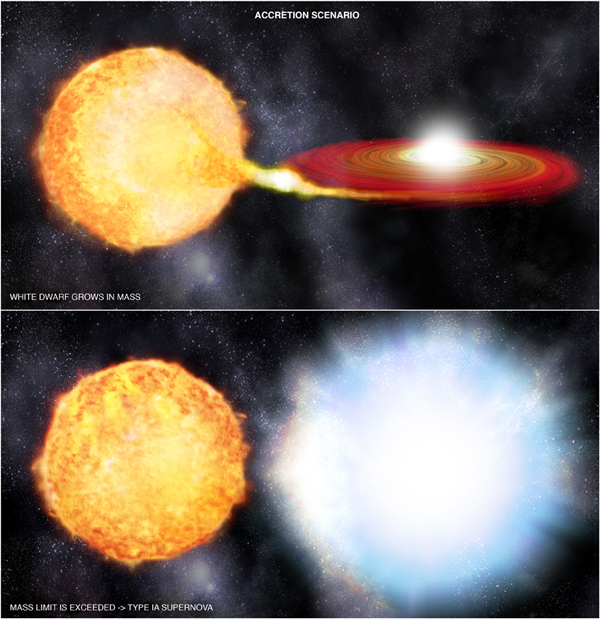
\includegraphics[width=0.3\textwidth]{figures/type_ia.jpg}}
                \put(60,0){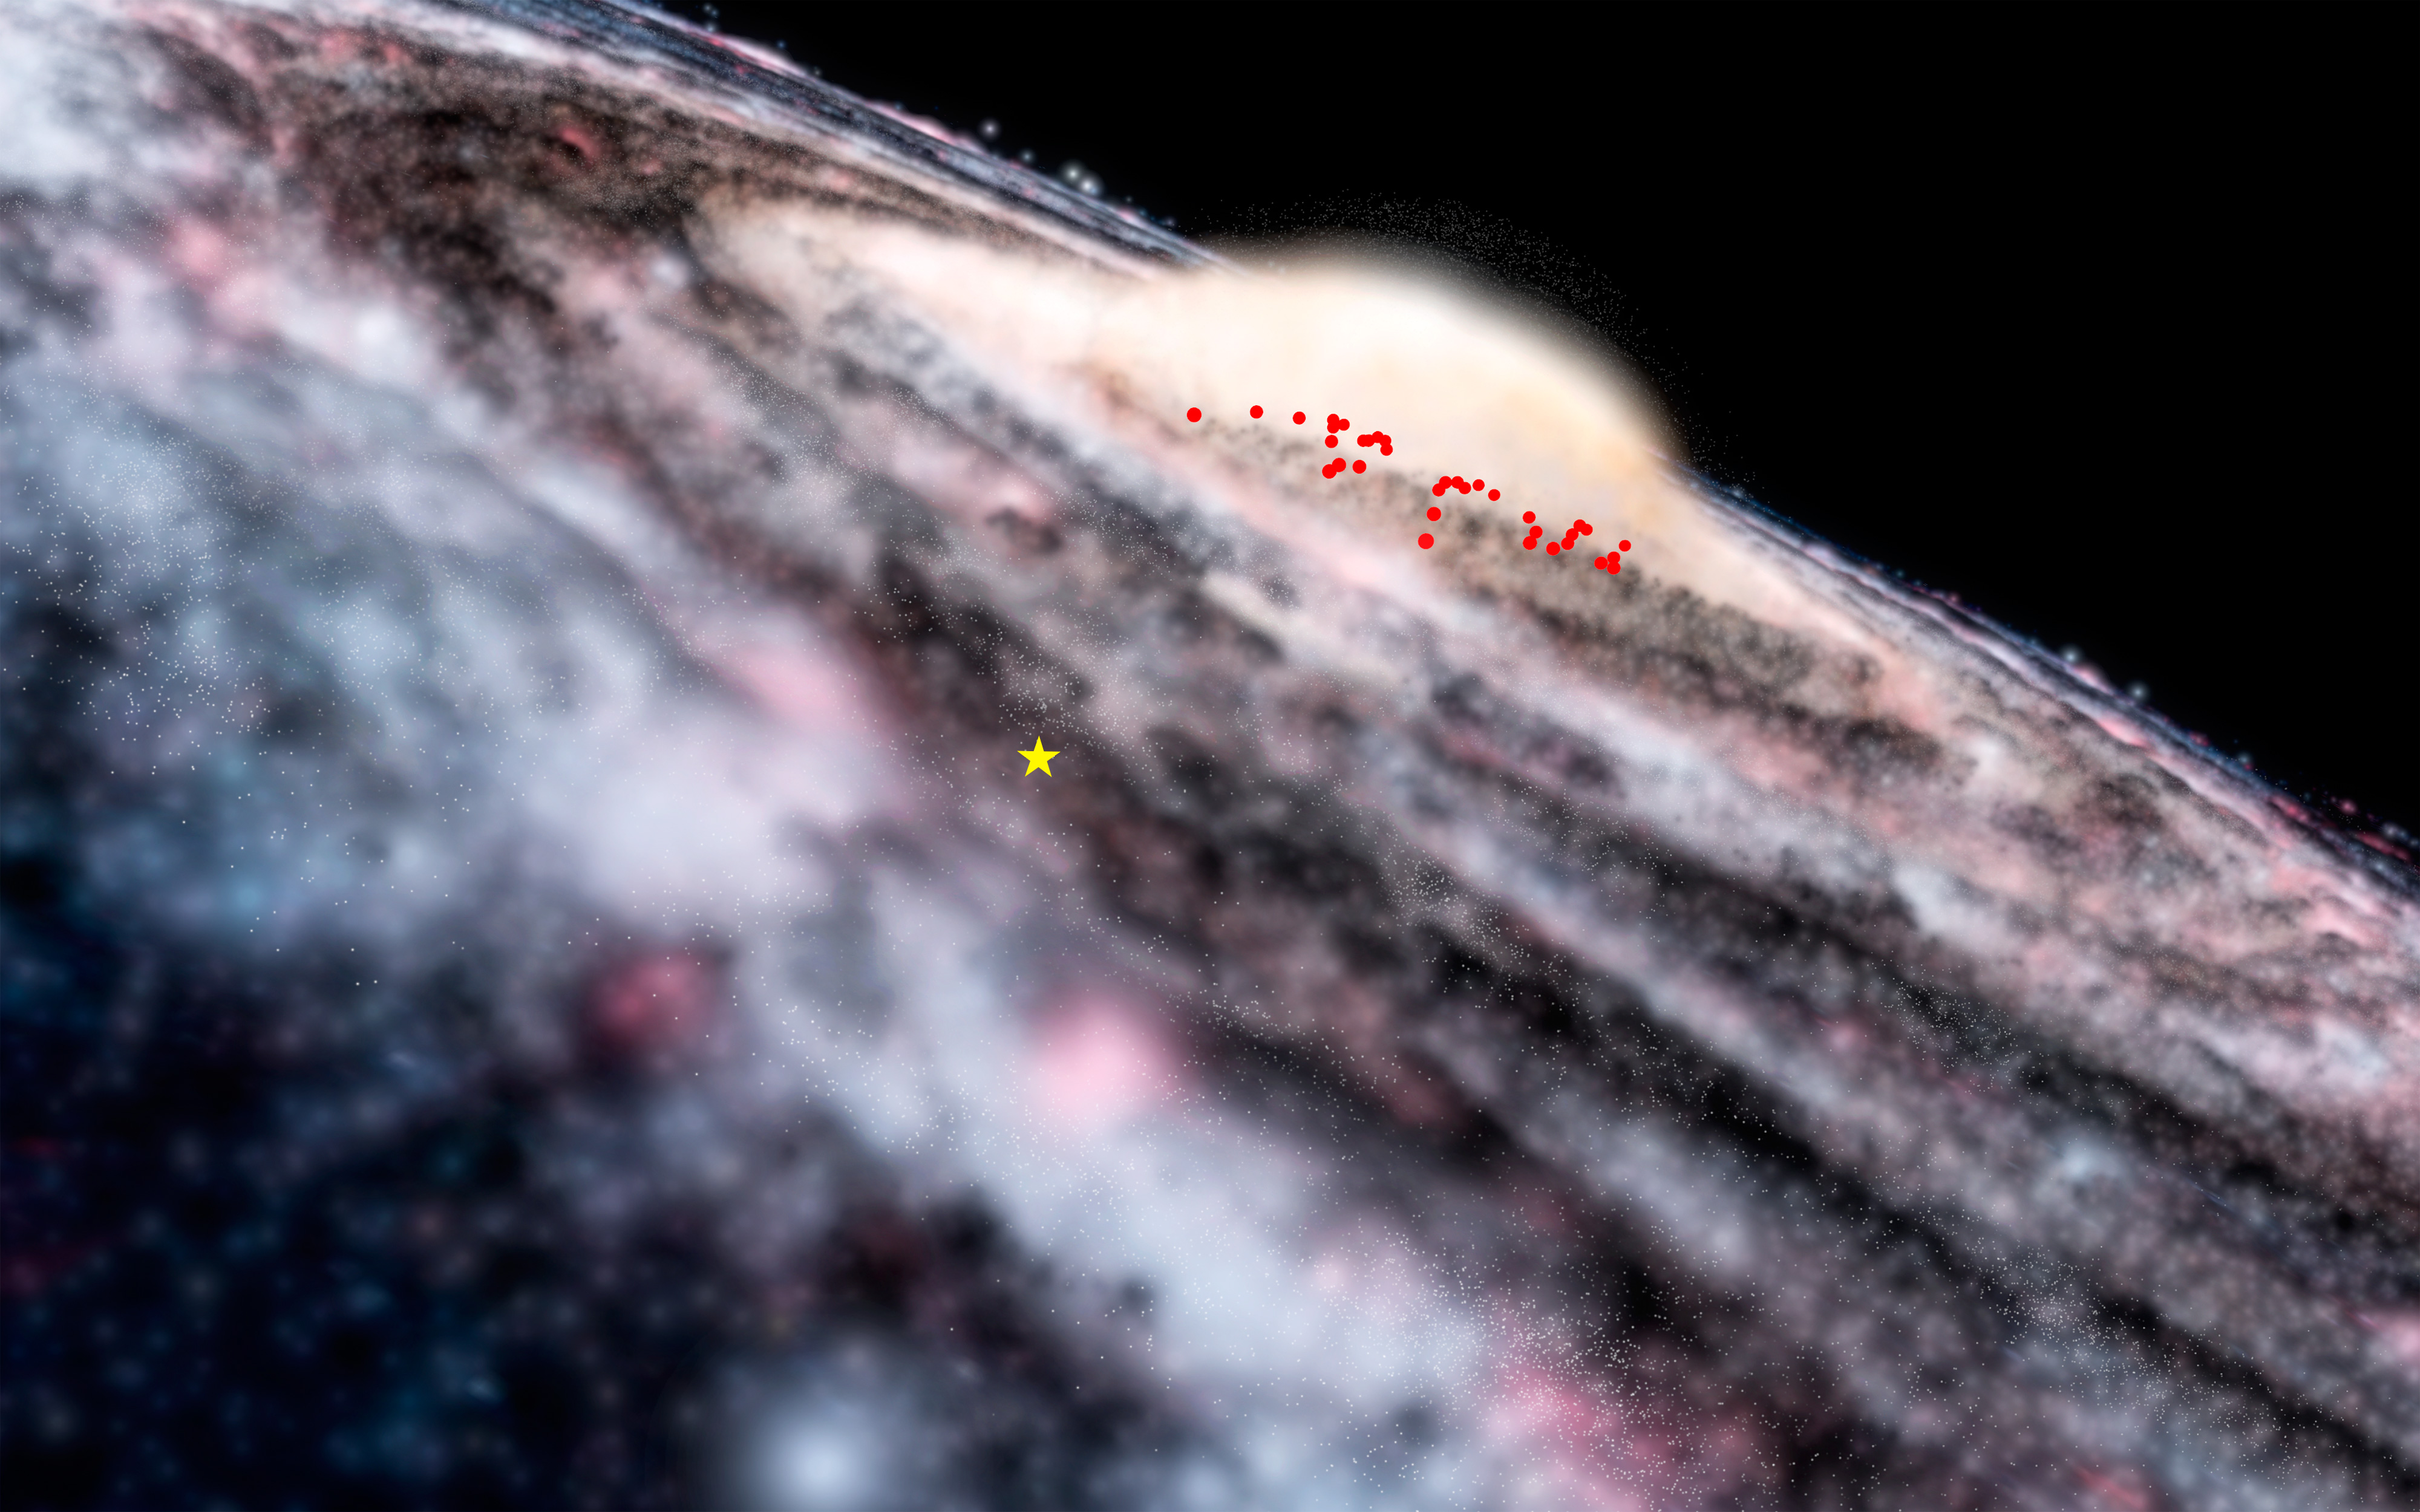
\includegraphics[width=0.4\textwidth]{figures/cepheid.jpg}}
                \put(70,25){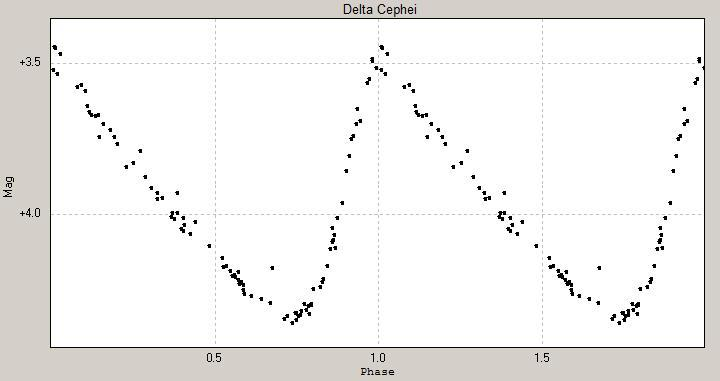
\includegraphics[width=0.3\textwidth]{figures/cepheid_curve.jpg}}
            \end{overpic}
        }
    \end{columns}
\end{frame}

\begin{frame}
    \frametitle{Standard Rulers}
    \begin{columns}
        \column{0.55\textwidth}
        \begin{itemize}
            \item Standard Rulers: Objects with known physical size.
\item CMB: Cosmic Microwave Background, fluctuations give a standard ruler at z$\sim$1100. \hfill \doi{10.1086/186504}
            \item BAO: Baryon Acoustic Oscillations, sound waves in early universe imprint a standard ruler on galaxy distribution. \hfill \arxiv{1201.2434}
            \item Strong lensing: Time delays between multiple images of a lensed object constrain distances. \hfill \doi{10.1093/mnras/128.4.307}
            \item Weak lensing: Distortion of galaxy shapes by intervening matter constrains the matter distribution.
        \end{itemize}
        \column{0.45\textwidth}
        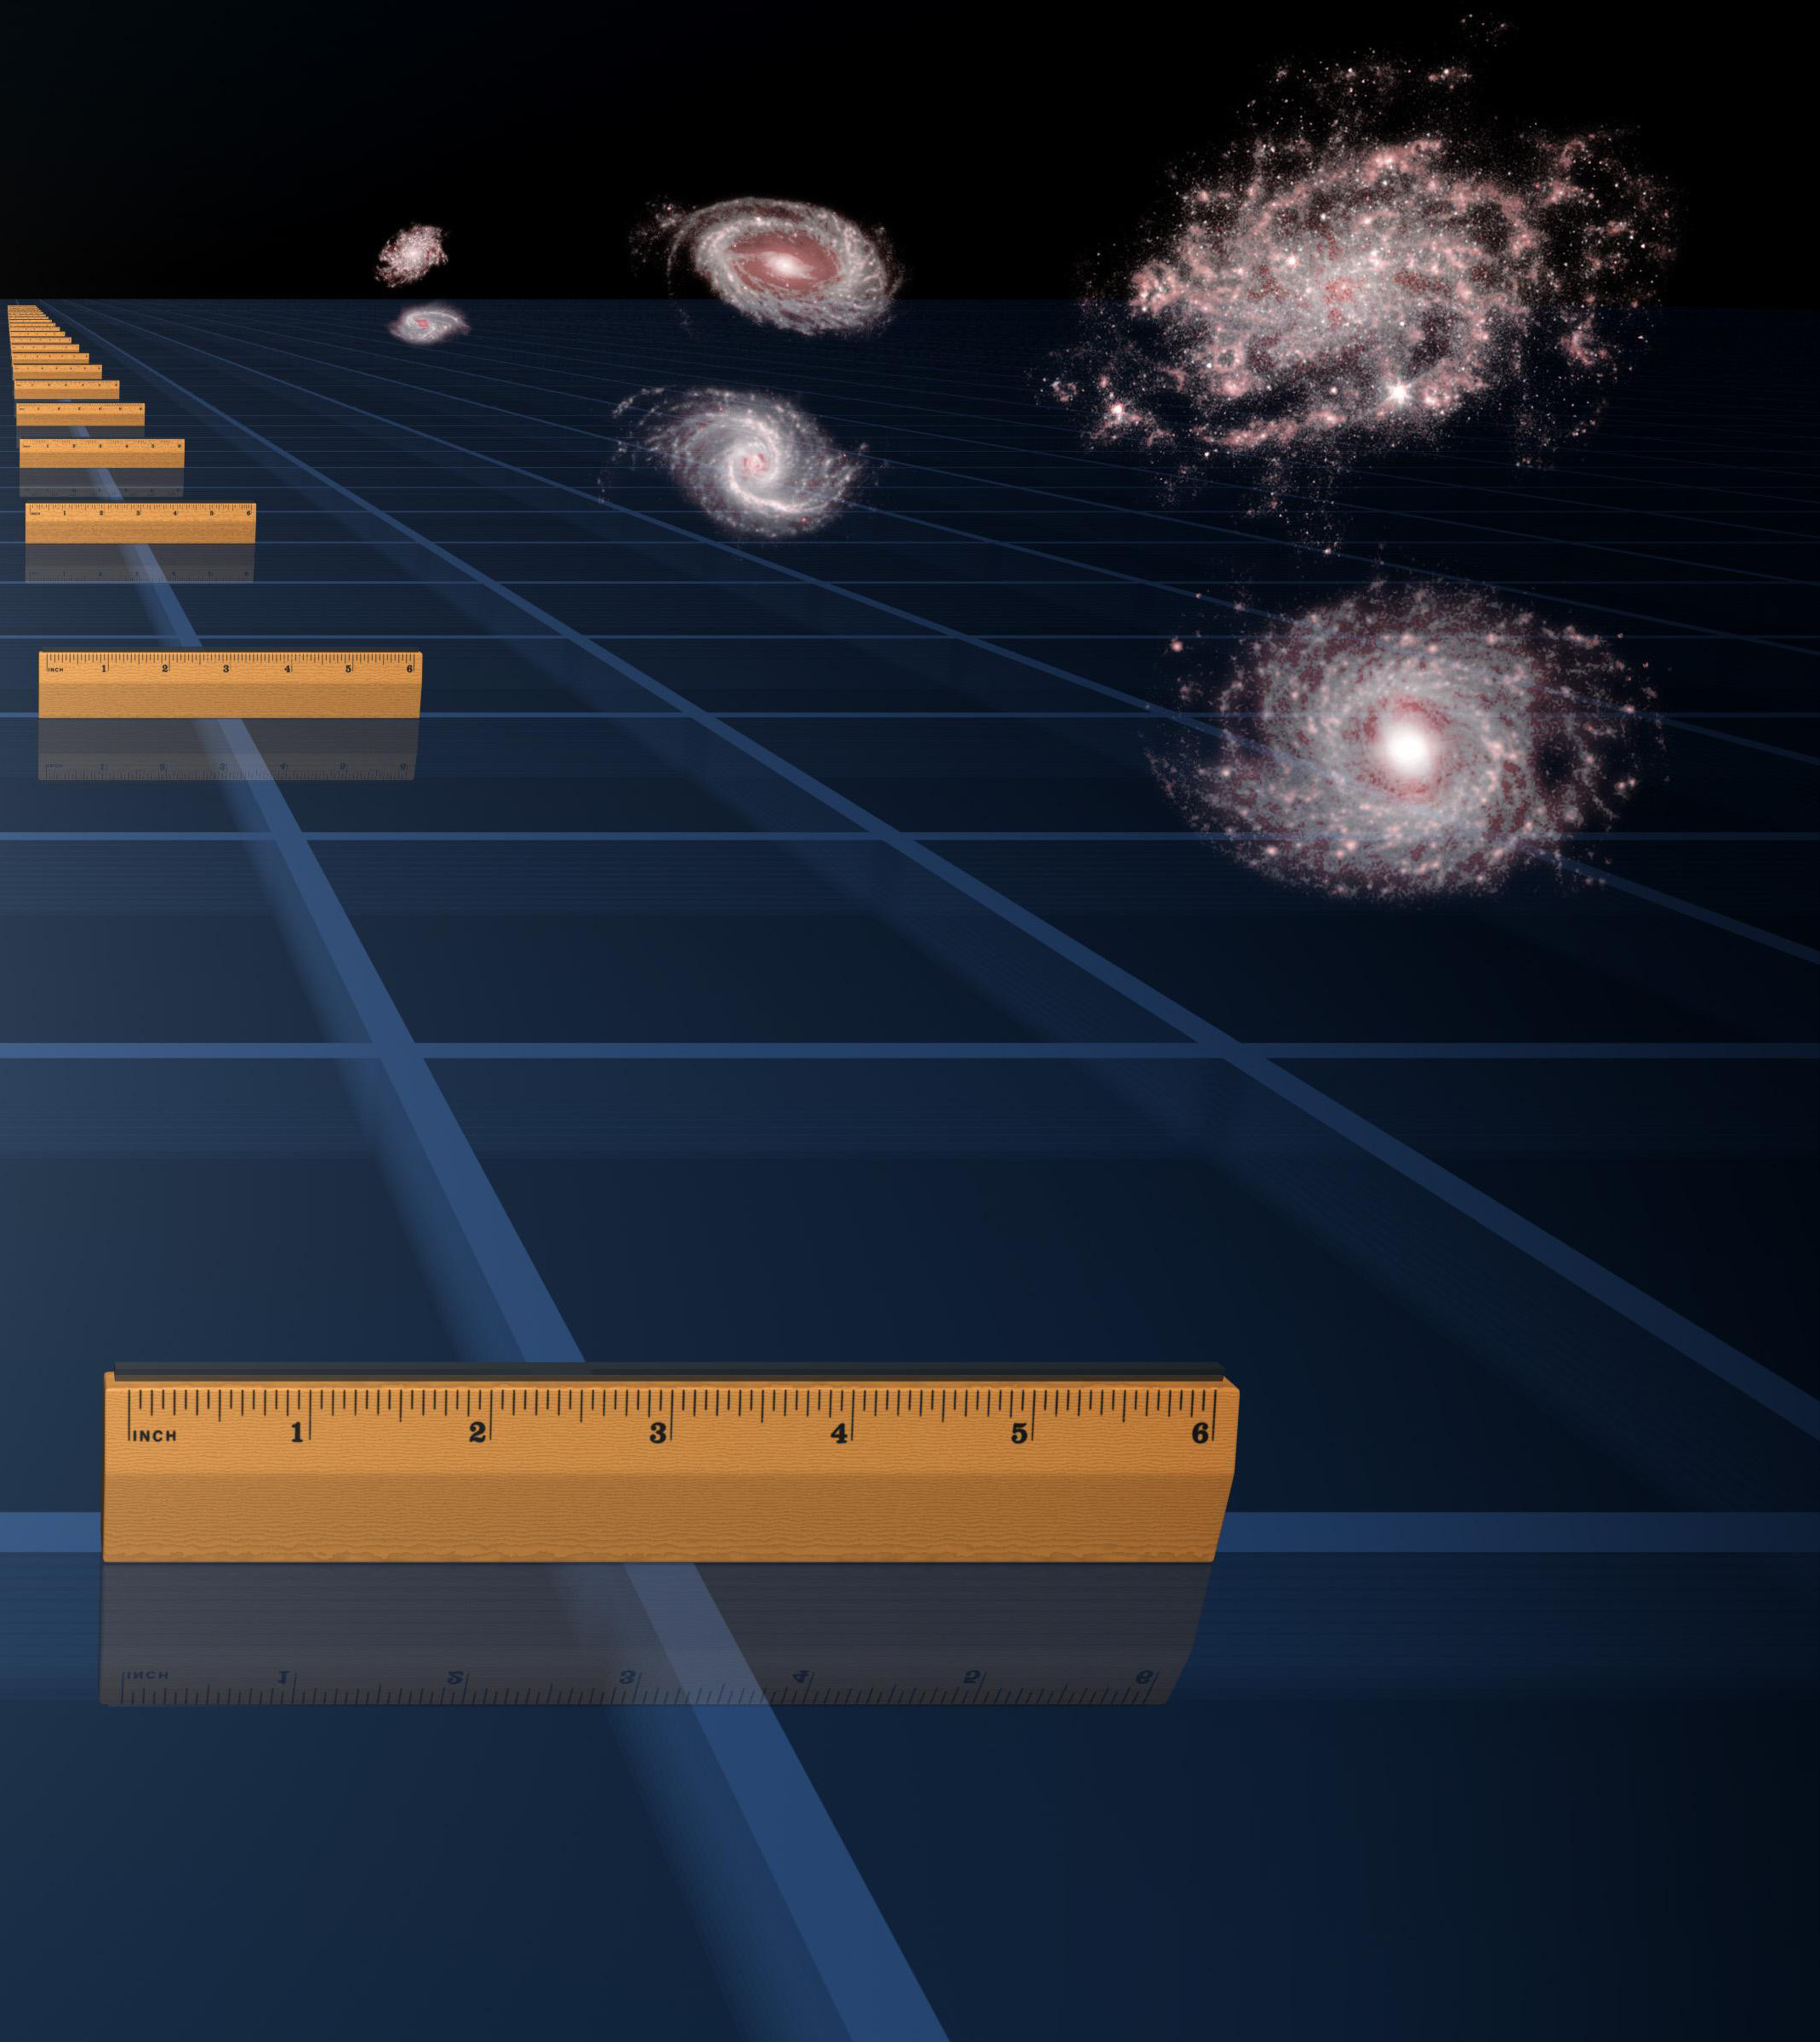
\includegraphics[width=\textwidth]{figures/rulers.jpg}
    \end{columns}
\end{frame}

\begin{frame}
    \frametitle{Standard Rulers}
    \framesubtitle{The cosmic microwave background}
    \begin{columns}
        \column{0.55\textwidth}
        \begin{itemize}
            \item CMB:  "Surface of last scattering" at $z\sim1100$.  Angular size of hot/cold spots gives a standard ruler. \hfill \doi{10.1086/186504}
            \item Temperature fluctuations: $\Delta T/T \sim 10^{-5}$.  \hfill \doi{10.1086/186504} 
            \item  Polarization: E and B modes.  B-modes from primordial gravitational waves are a key target.
        \end{itemize}
        \column{0.45\textwidth}
        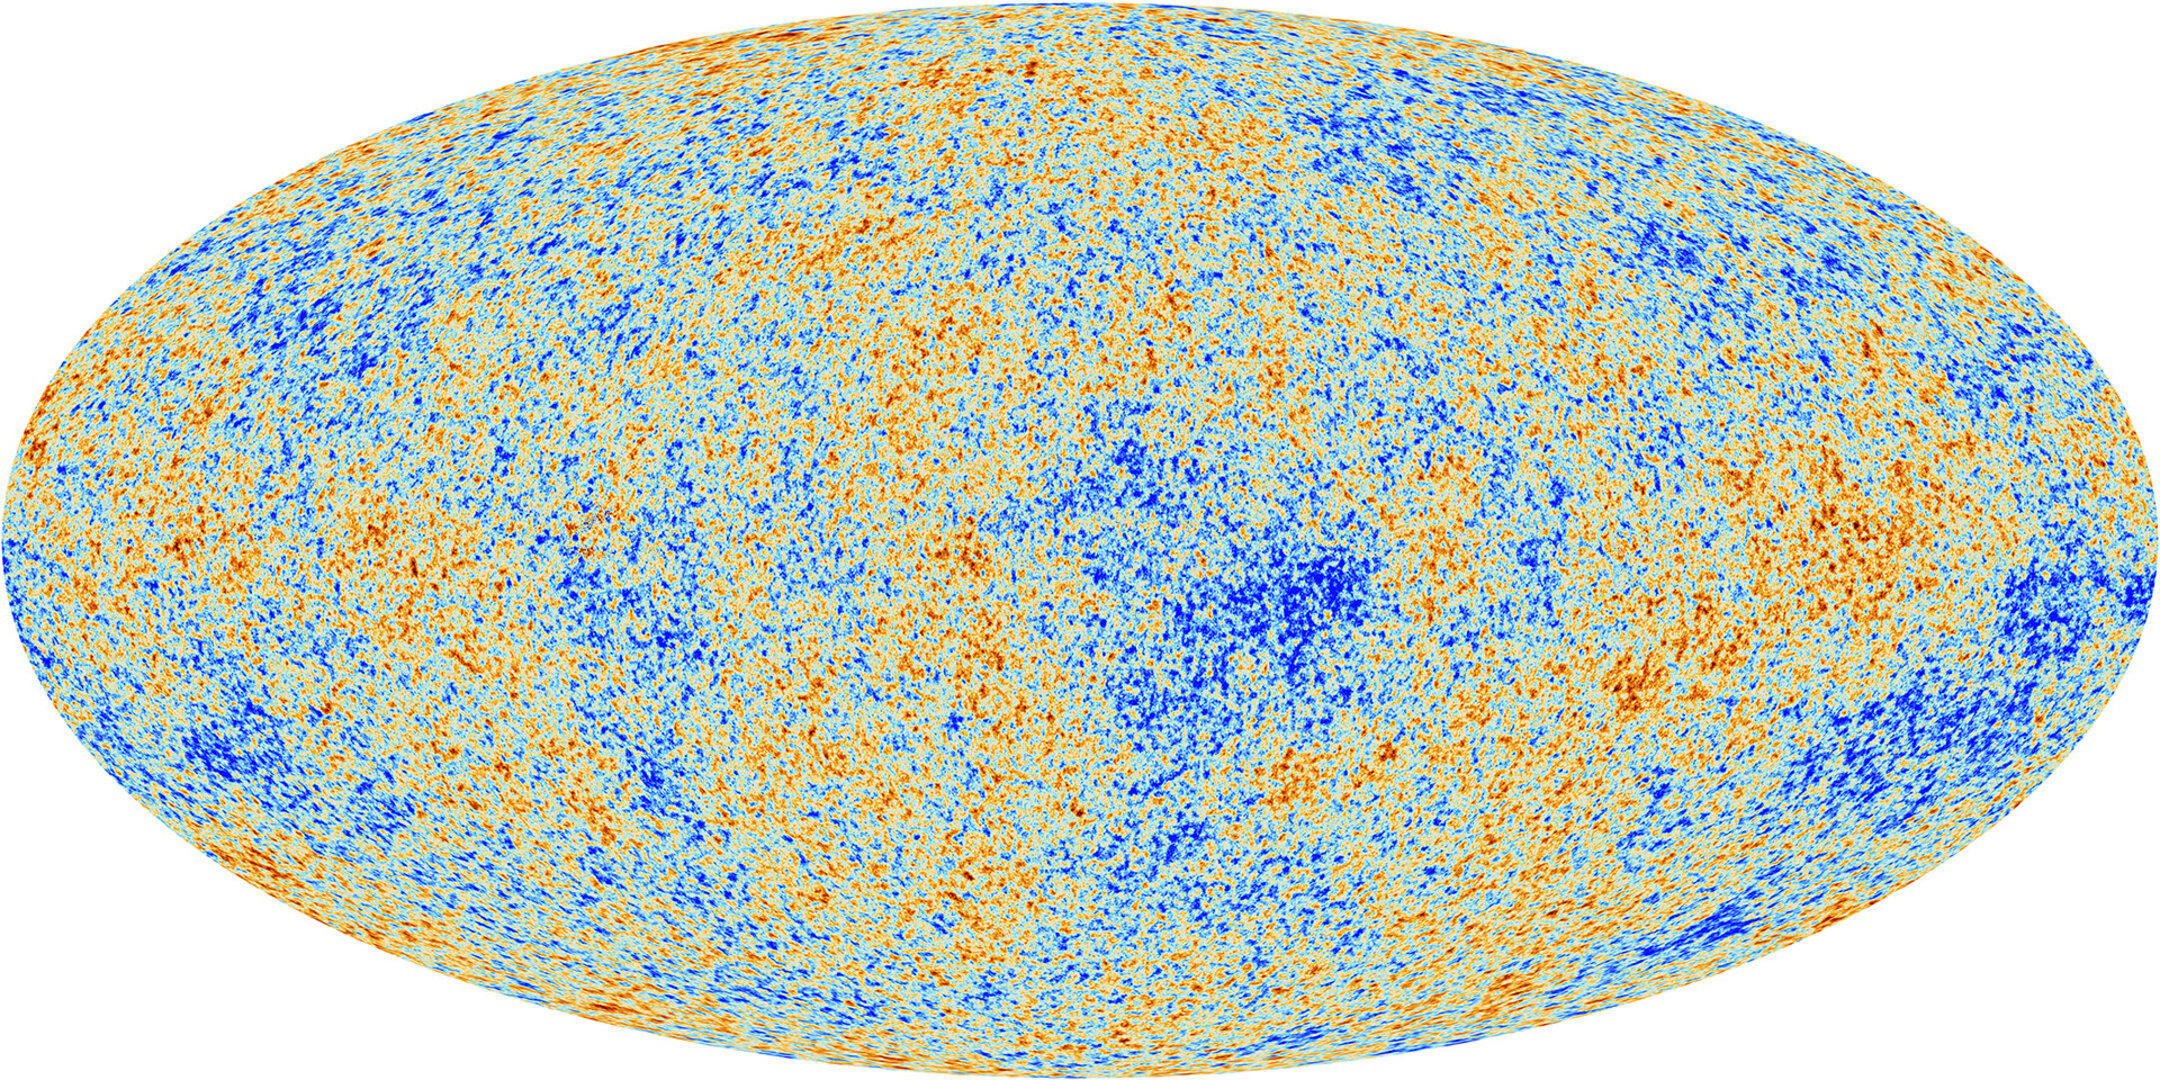
\includegraphics[width=\textwidth]{figures/cmb.png}
        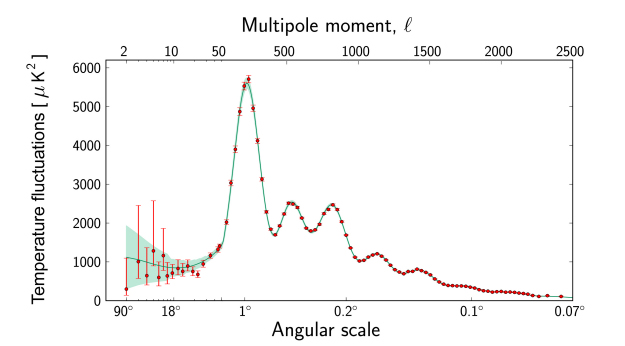
\includegraphics[width=\textwidth]{figures/cmb_power_spectrum.jpg}%
    \end{columns}
\end{frame}

\begin{frame}
    \frametitle{Standard Rulers}
    \framesubtitle{Baryon Acoustic Oscillations}
    \begin{columns}
        \column{0.58\textwidth}
        \begin{itemize}
            \item BAO: Sound waves in the early Universe imprint a characteristic scale on the distribution of baryons (and galaxies). \hfill \arxiv{1201.2434}
            \item SDSS: Sloan Digital Sky Survey, one of the first surveys to measure BAO. \hfill \oldarxiv{astro-ph/0501171}
            \item DESI: Dark Energy Spectroscopic Instrument, current best BAO measurements. \hfill \arxiv{2404.03001}
        \end{itemize}
        \column{0.42\textwidth}
        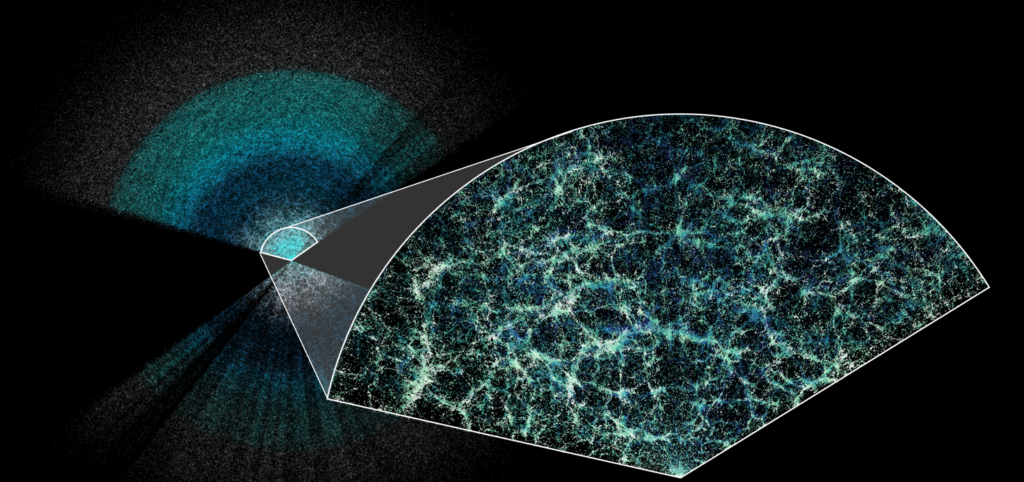
\includegraphics[width=\textwidth]{figures/desi_galaxies.png}
        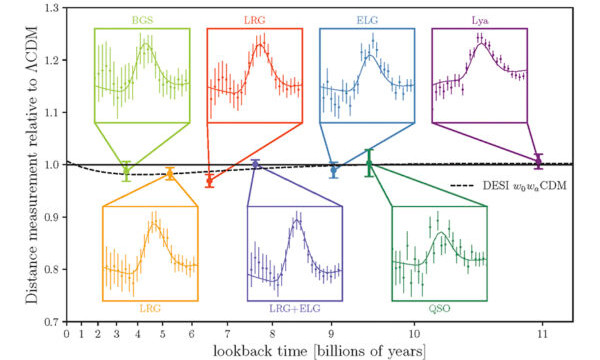
\includegraphics[width=\textwidth]{figures/desi_bao.jpg}%
    \end{columns}
\end{frame}

\begin{frame}
    \frametitle{Standard Rulers}
    \framesubtitle{Strong Lensing}
    \begin{columns}
        \column{0.55\textwidth}
        \begin{itemize}
            \item Strong Lensing: Light from a distant object is bent by the gravity of a massive foreground object (e.g., a galaxy or galaxy cluster). \hfill \doi{10.1093/mnras/128.4.307}
            \item Time Delays: Differences in path lengths of multiple images lead to time delays, which can be used to measure distances. \hfill \arxiv{2210.15794}
        \end{itemize}
        \column{0.45\textwidth}
        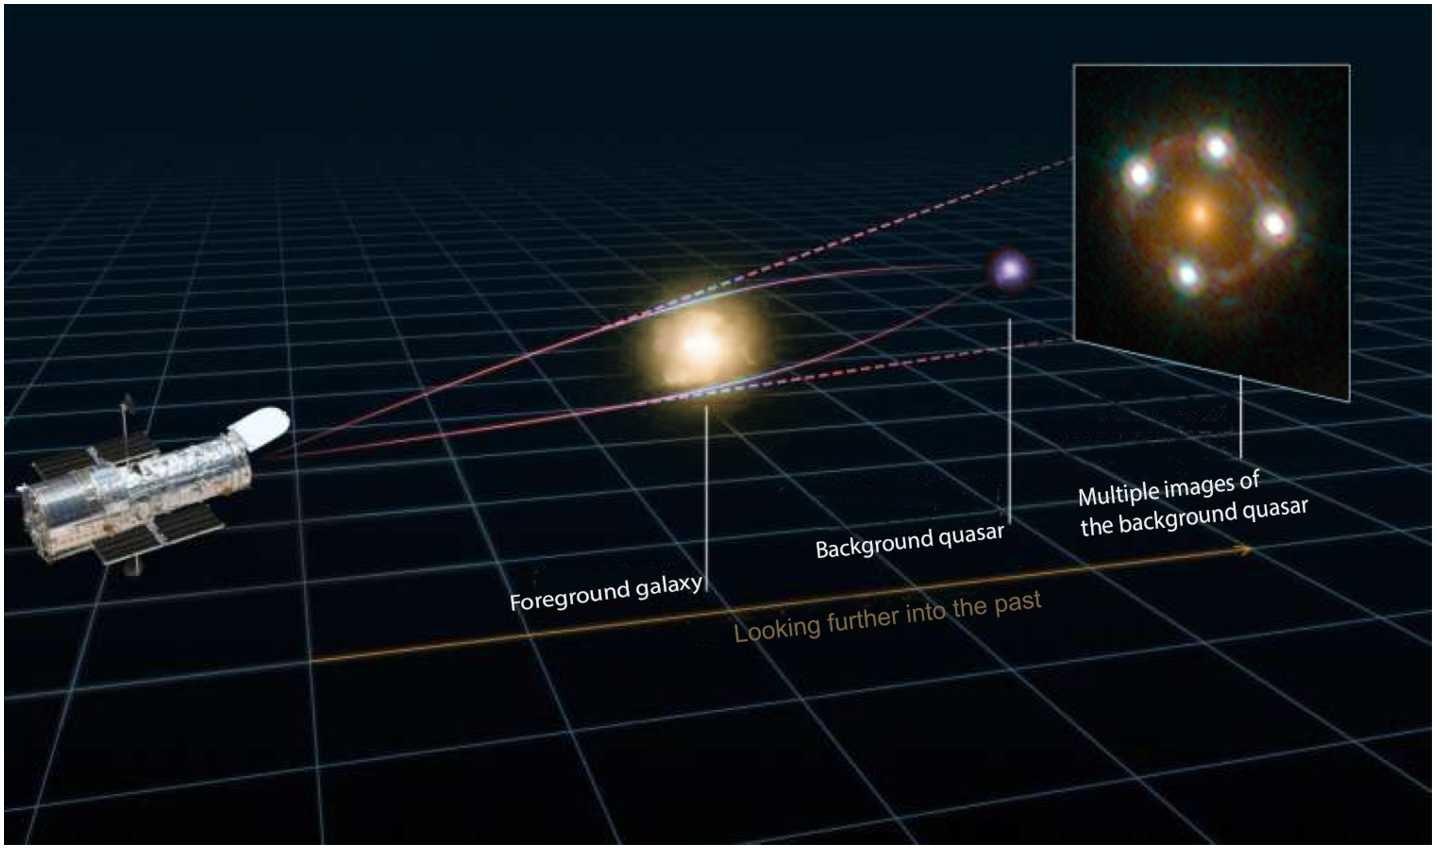
\includegraphics[width=\textwidth]{figures/time_delay.jpg}
        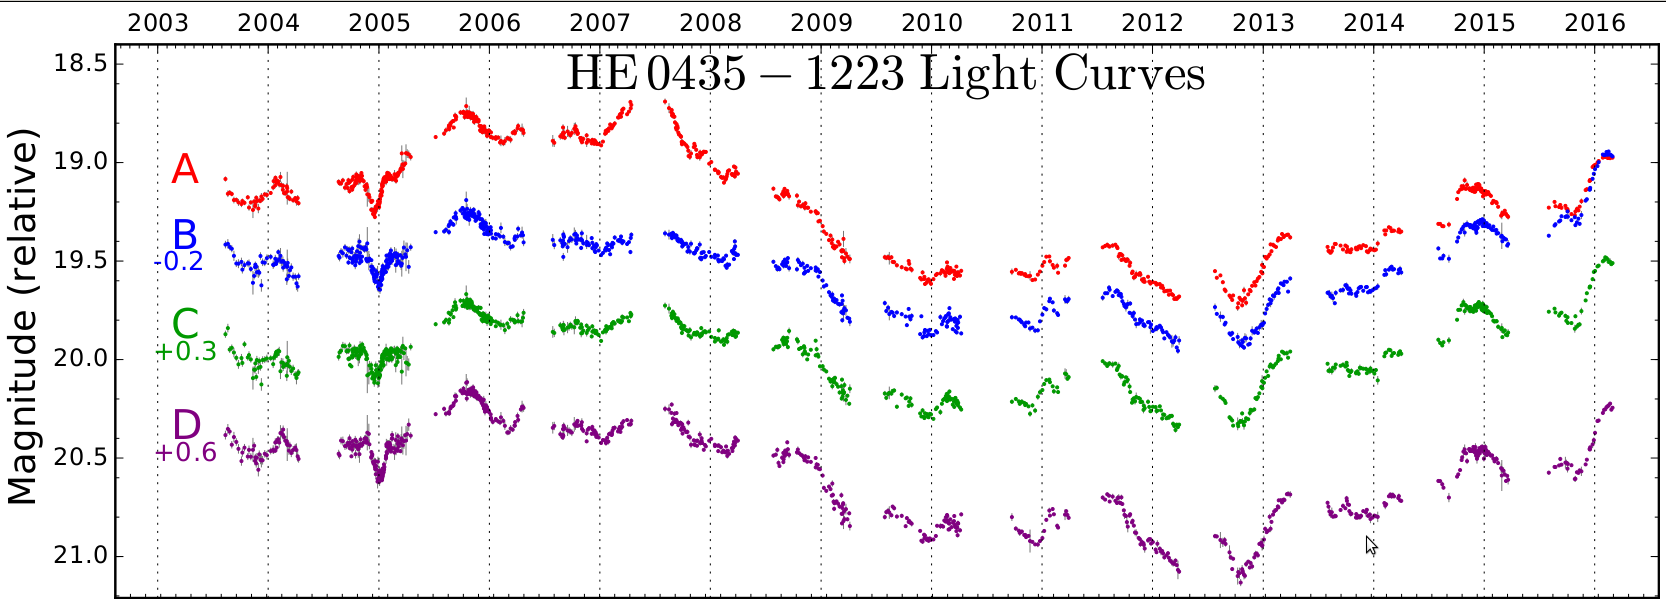
\includegraphics[width=\textwidth]{figures/time_delay_curve.png}%
    \end{columns}
\end{frame}

\begin{frame}
    \frametitle{Standard Rulers}
    \framesubtitle{Weak Lensing}
    \begin{columns}
        \column{0.55\textwidth}
        \begin{itemize}
            \item Weak Lensing:  Small distortions in the shapes of background galaxies caused by the gravitational lensing of intervening matter.
            \item Surveys like DES, KiDS, and HSC have used weak lensing to map the distribution of dark matter. \hfill \arxiv{1610.04606}\arxiv{1910.05336}
        \end{itemize}
        \column{0.45\textwidth}
        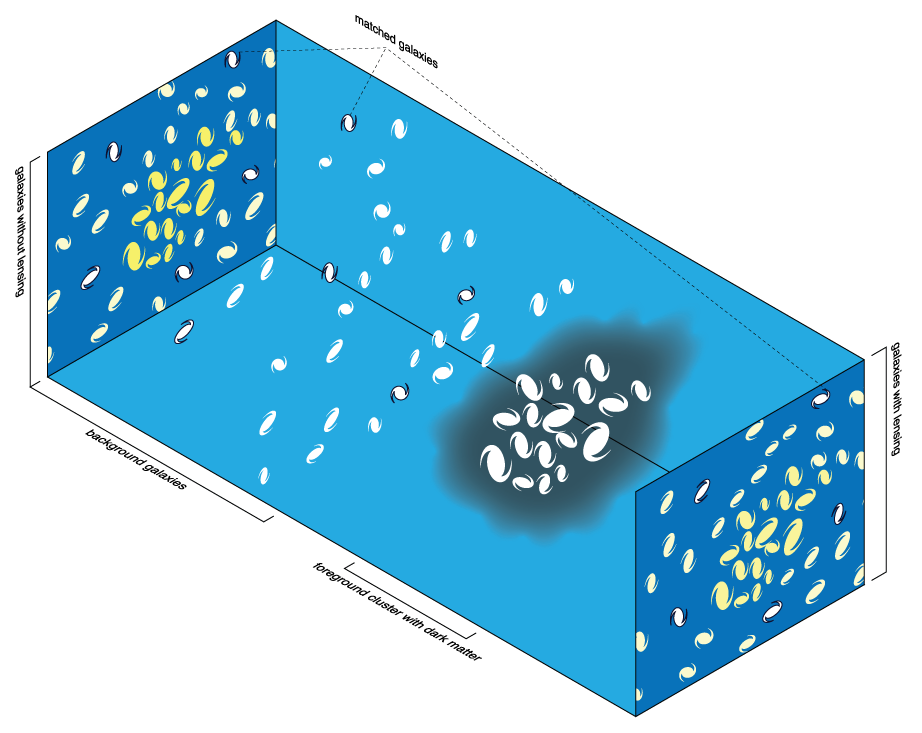
\includegraphics[width=\textwidth]{figures/weak_lensing.png}
    \end{columns}
\end{frame}

\begin{frame}
    \frametitle{Standard Sirens}
    \begin{columns}
        \column{0.5\textwidth}
        \begin{itemize}
            \item Standard Sirens: Gravitational wave sources with known intrinsic "loudness". \hfill \doi{10.1038/323310a0} \oldarxiv{astro-ph/0504616}
            \item Bright sirens: GW events with an electromagnetic counterpart, allowing redshift measurement. \hfill \arxiv{1710.05835}
            \item Dark sirens: GW events without an electromagnetic counterpart; statistical redshift information is used. \hfill \arxiv{1901.01540}
            \item Spectral sirens: Redshift is inferred statistically from the mass distribution of merging black holes. \hfill \arxiv{1908.09084}
        \end{itemize}
        
        \column{0.5\textwidth}
        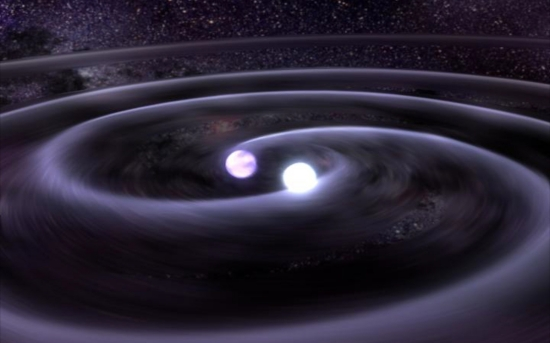
\includegraphics[height=0.33\textwidth]{figures/gw.jpg}%
        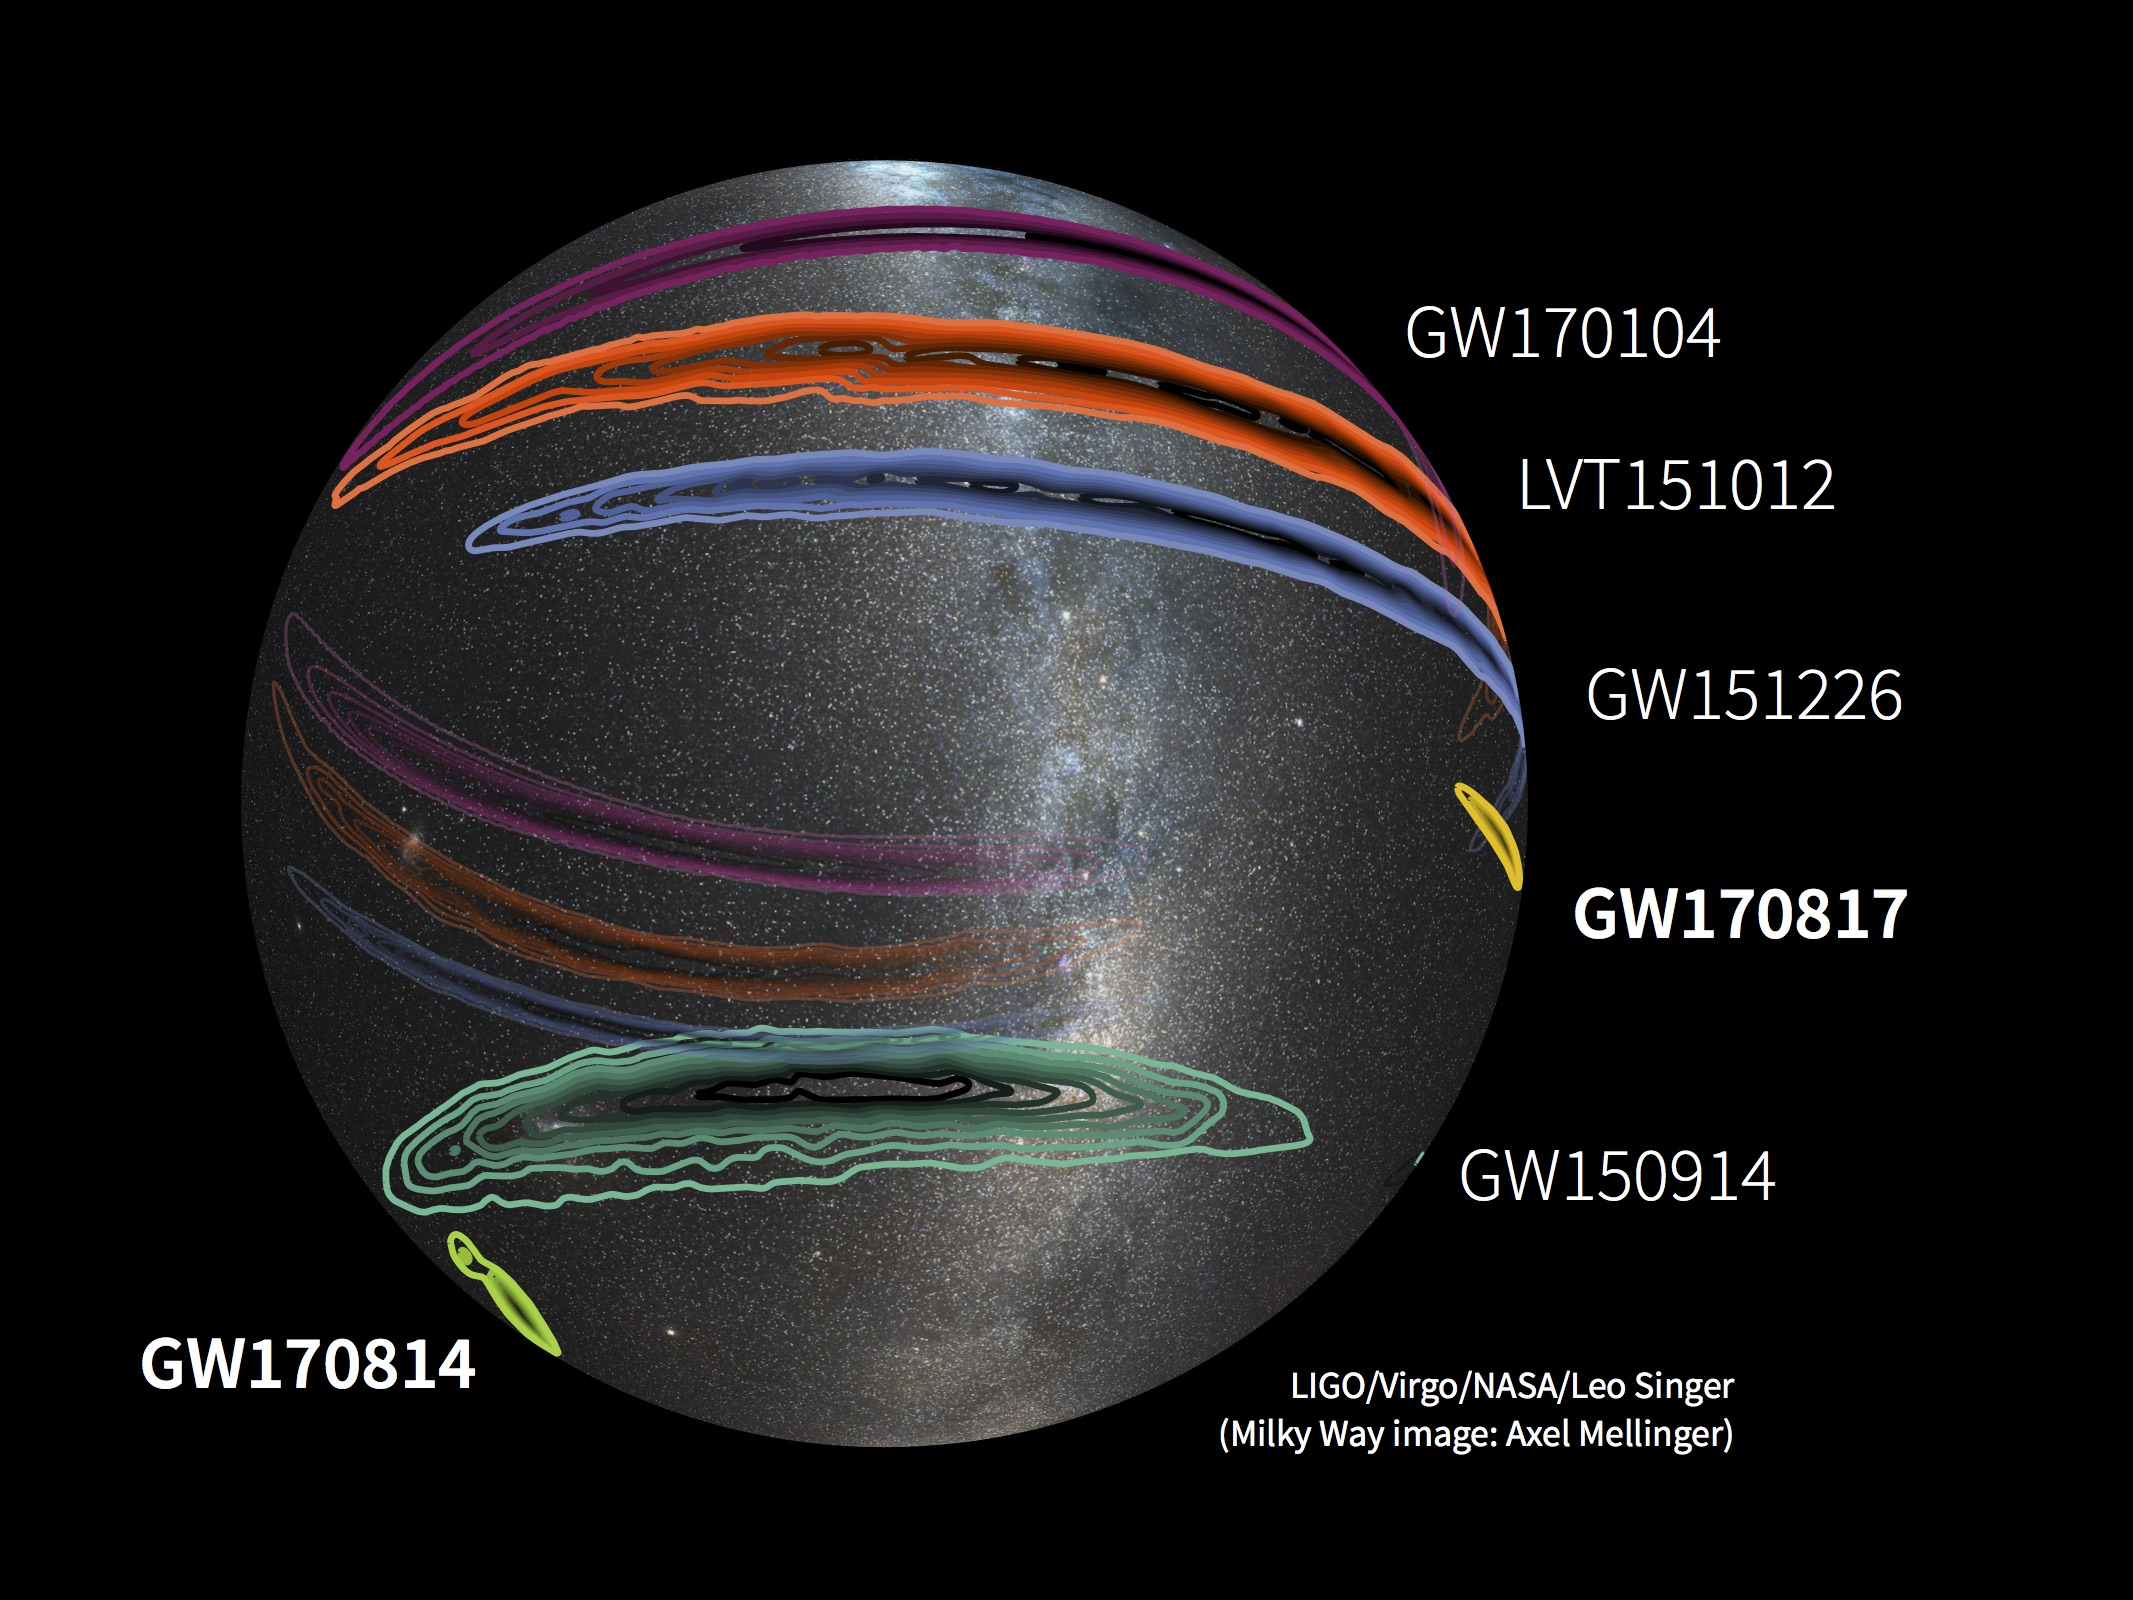
\includegraphics[height=0.33\textwidth]{figures/gw_local.jpg}
        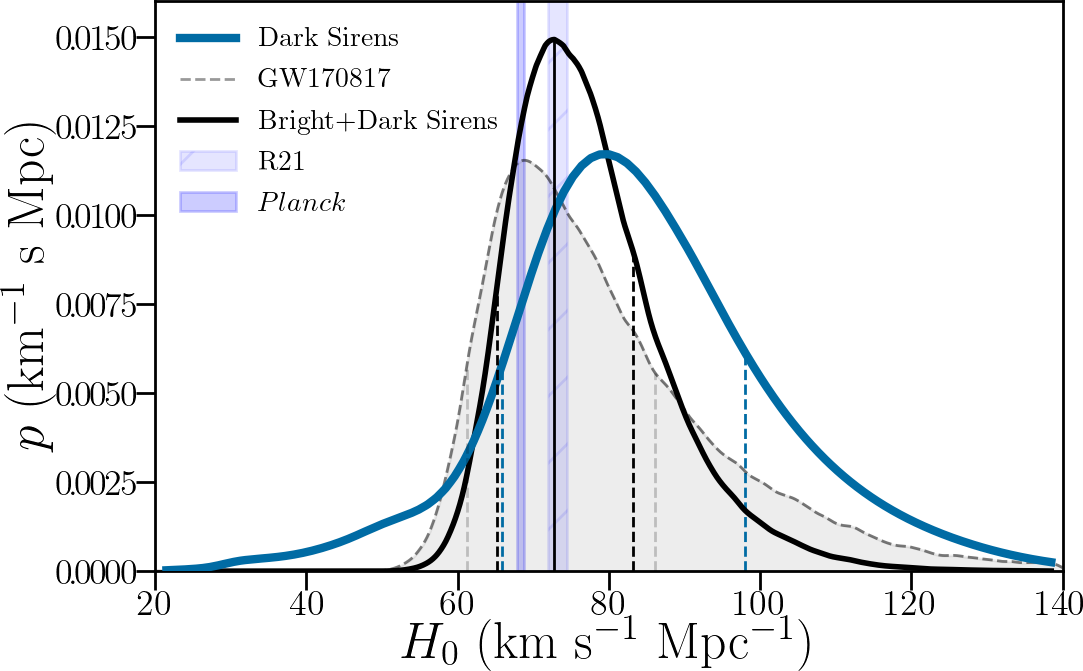
\includegraphics[width=\textwidth]{figures/posterior_O3_dr9beta_170817.png} % 2111.06445
        
    \end{columns}
\end{frame}

\begin{frame}
    \frametitle{Standard Clocks}
    \begin{columns}
        \column{0.5\textwidth}
        \begin{itemize}
            \item Standard Clocks: Objects or phenomena whose time evolution can be used to measure time or distances.
            \item Cosmic Chronometers: Passively evolving galaxies whose age can be measured, giving $dH/dz$. \hfill \oldarxiv{astro-ph/0106145}
            \item Pulsar timing arrays: Variations in the arrival times of pulsar signals can be used to detect gravitational waves and measure distances.
        \end{itemize}
        \column{0.5\textwidth}
        %\includegraphics[width=\textwidth]{figures/clocks.jpg}
        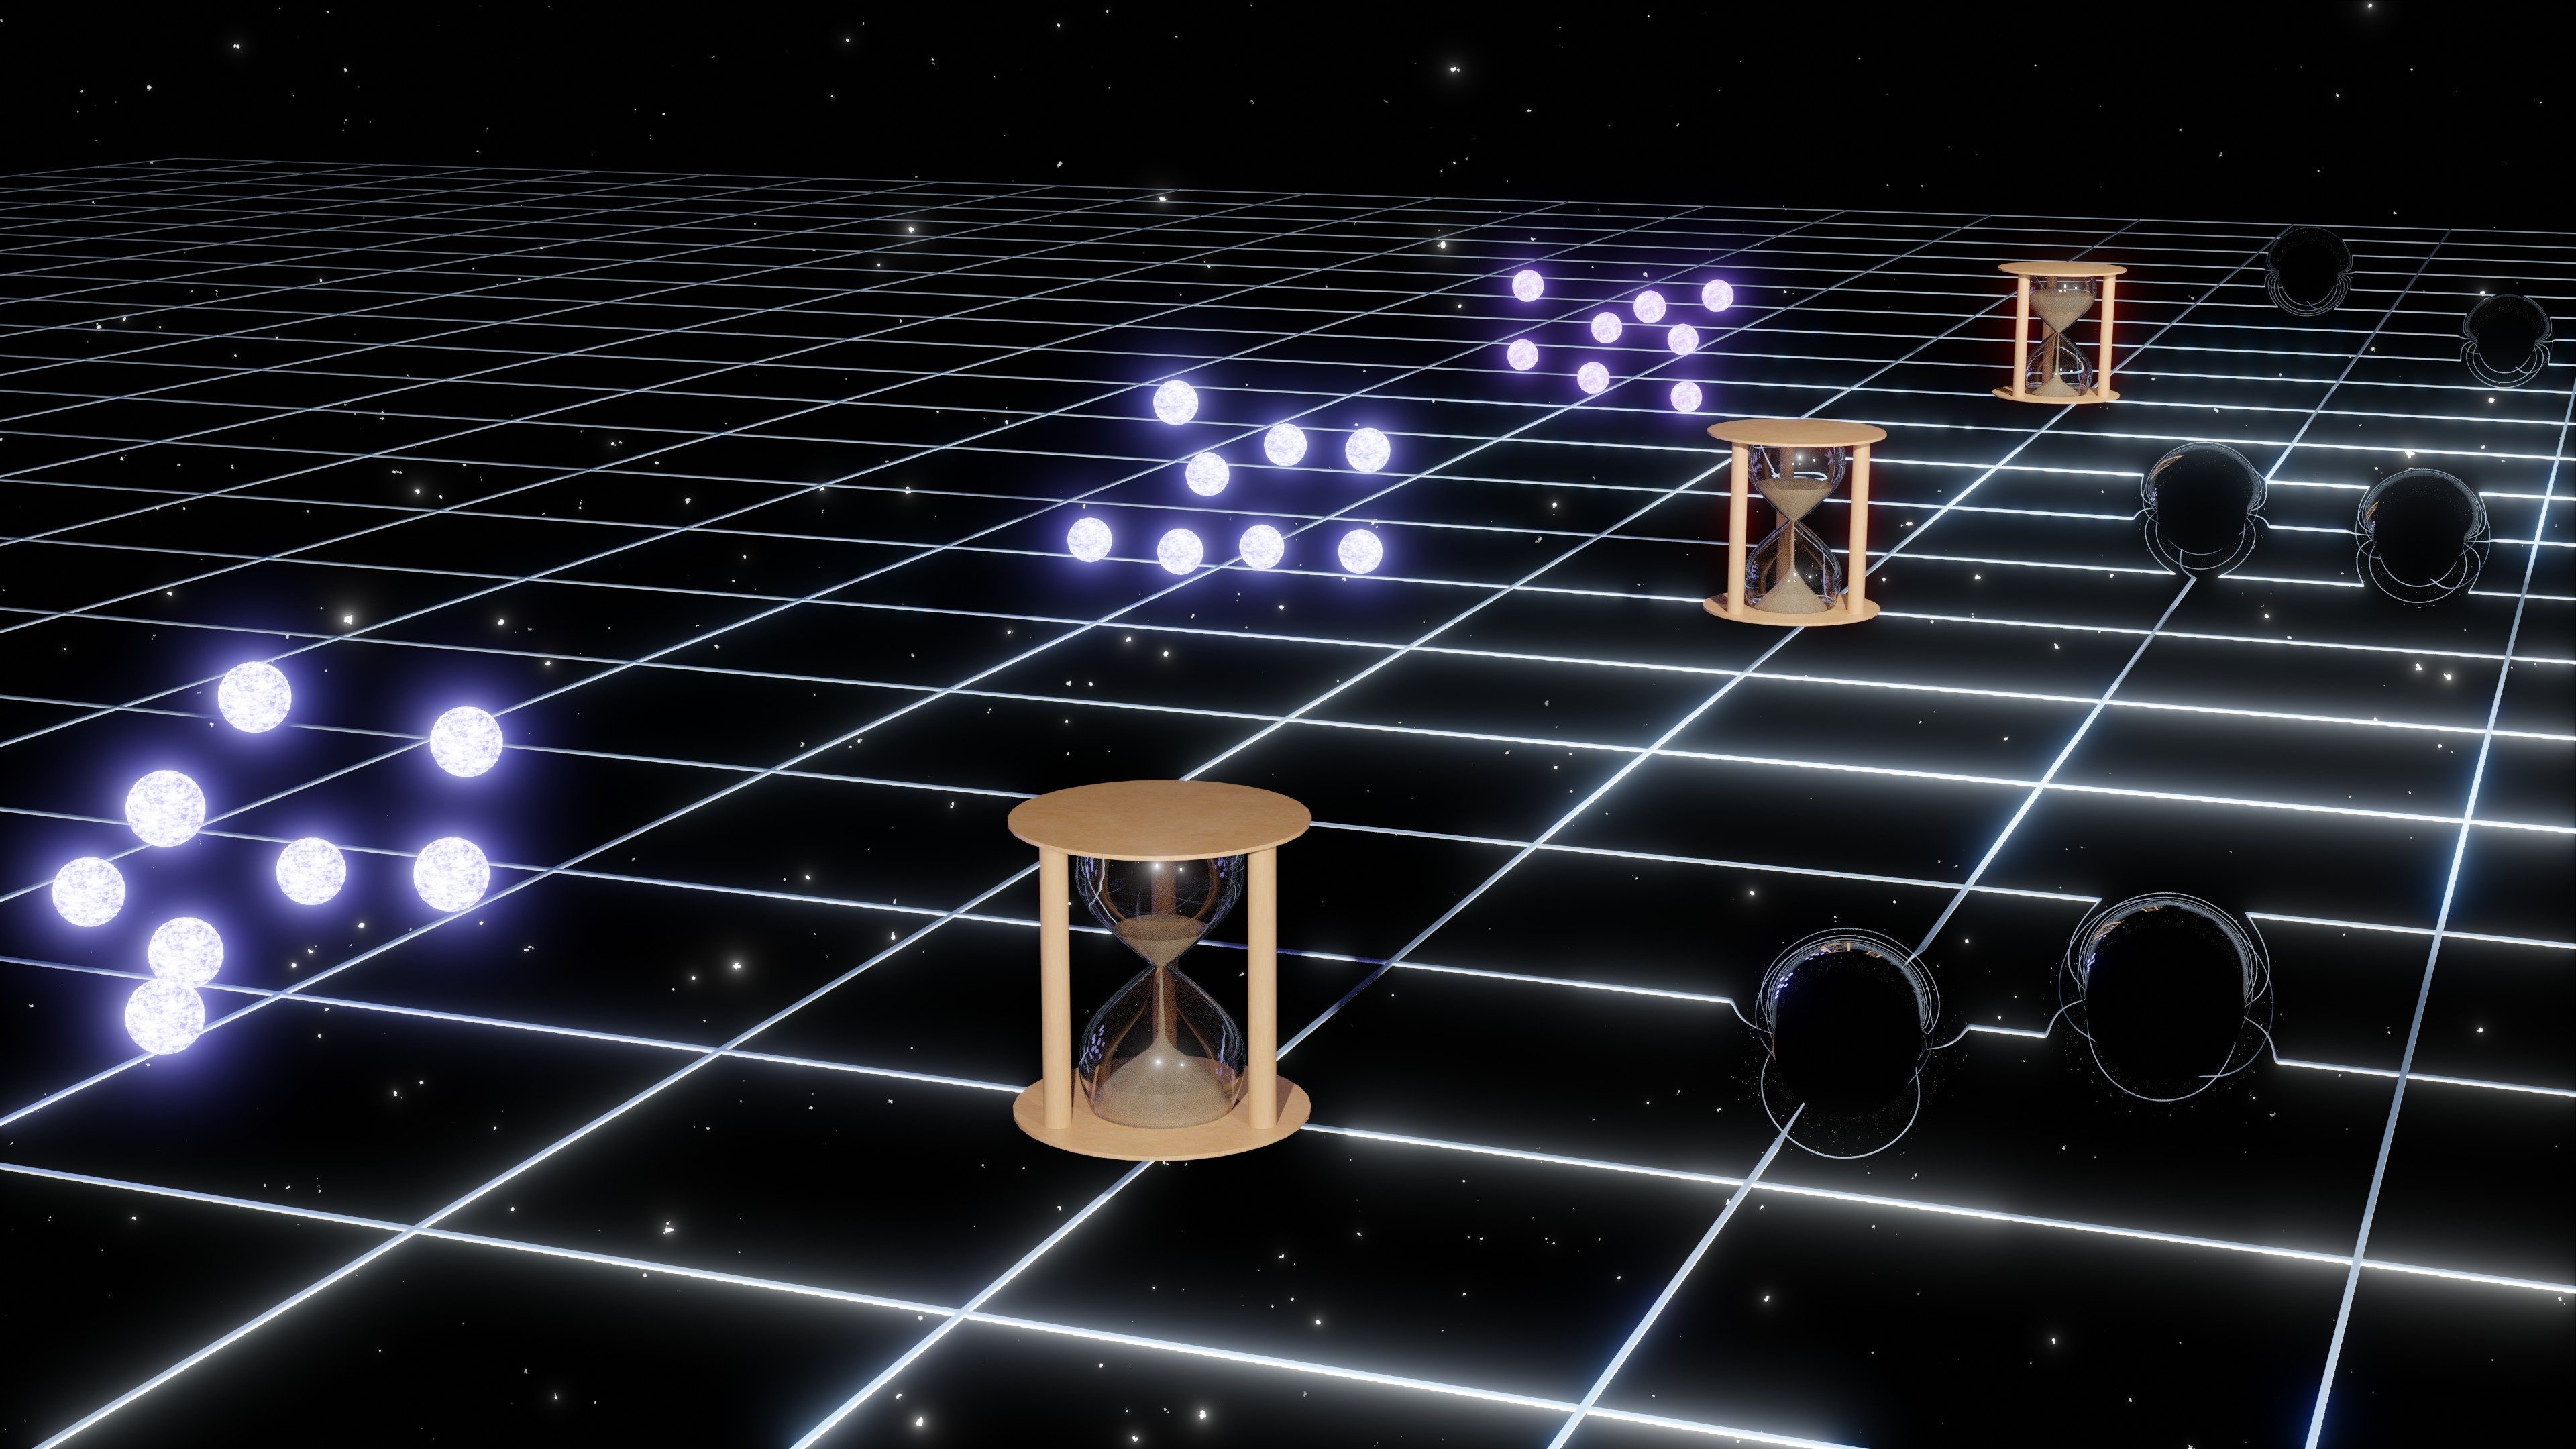
\includegraphics[width=\textwidth]{figures/timers.jpg}
        %\includegraphics[width=\textwidth]{figures/cosmic_chronometers.png}
        %\includegraphics[width=\textwidth]{figures/pulsar_timing_array.jpg}
    \end{columns}
\end{frame}
 
\begin{frame}
    \frametitle{The Hubble tension}
    \begin{columns}
        \column{0.5\textwidth}
        \begin{itemize}
            \item CMB: $H_0=67.4\pm0.5$ km/s/Mpc. \hfill \arxiv{1807.06209}
            \item S$H_0$ES: $H_0=73.2\pm1.3$ km/s/Mpc. \hfill \arxiv{2112.04510}
            \item Exciting if not measurement error
                \begin{itemize}
                    \item People trust the CMB measurement, but perhaps not the $\Lambda$CDM model assumptions.
                    \item Measurements of $H_0$ from supernovae are notoriously challenging (crowding, dust, metallicity, etc.)
                \end{itemize}
            \item As of 2024, Hubble three ways (Cepheids, TRGB, JAGB) show some convergence:
                \begin{description}
                    \item [CCHP (Freedman)] \hfill$(72.0, 69.8, 67.96)\pm1.8$
                    \item [SH0ES (Riess)] \hfill$(73.4, 72.1, 72.2)\pm2.2$
                \end{description}                                      
                \hfill\arxiv{2408.06153}\arxiv{2408.11770}
        \end{itemize}
        \column{0.5\textwidth}
        \includegraphics<1>[width=\textwidth]{figures/H0_1.jpg}%
        \includegraphics<2>[width=\textwidth]{figures/H0_2.jpg}%
        \includegraphics<3>[width=\textwidth]{figures/H0_3.png}%
        \includegraphics<4>[width=\textwidth]{figures/H0_4.png}%
        \only<5>{
            \begin{overpic}[height=0.9\textheight]{figures/hH0whisker_Chapter2_SameRowColor4_SN_P15.pdf}
                \put(18,4){\tiny\arxiv{2103.01183}}
            \end{overpic}
        }
    \end{columns}
\end{frame}

\begin{frame}
    \frametitle{The $S_8$ tension}
    \framesubtitle{aka $\sigma_8$/weak lensing tension}
    \begin{columns}
        \column{0.52\textwidth}
        \begin{itemize}
            \item $S_8$ quantifies the amplitude of matter fluctuations on large scales.
            \item $S_8=\sigma_8(\Omega_m/0.3)^{0.5}$.
            \item CMB: $S_8 \approx 0.834$. \hfill \arxiv{1807.06209}
            \item Weak lensing:  $S_8 \approx 0.76$. \hfill \arxiv{1610.04606}\arxiv{1910.05336}
            \item Tension at the $2-3\sigma$ level.
            \item Possible systematics in weak lensing or new physics?
        \end{itemize}
        \column{0.48\textwidth}
         \includegraphics<1>[width=\textwidth]{figures/K+Dcontour_sig8om.pdf}%
        \includegraphics<2>[width=\textwidth]{figures/K+Dcontour.pdf}%
        \only<3>{%
        \begin{overpic}[width=\textwidth]{figures/s8_tension.pdf}
            \put(0,0){\arxiv{2402.08458}}
        \end{overpic}}
    \end{columns}
    \hfill\arxiv{2305.17173}
\end{frame}

\begin{frame}
    \frametitle{Other Tensions and Anomalies}
    \begin{columns}
        \column{0.5\textwidth}
        \begin{itemize}
            \item $A_{\rm lens}$ anomaly: CMB lensing amplitude higher than expected. \hfill \arxiv{1807.06209}
            \item Non-zero curvature: Some data hints at a closed universe. \hfill \arxiv{1902.04029}
            \item CMB anisotropic anomalies:  Large-scale features that challenge statistical isotropy. \hfill \arxiv{1510.07929}
            \item BBN anomalies: Discrepancies in light element abundances. \hfill \arxiv{1912.01132}
        \end{itemize}
        \column{0.5\textwidth}
        \begin{overpic}[width=\textwidth]{figures/omegak_H0.pdf} 
            \put(0,0){\tiny\arxiv{1908.09139}}
        \end{overpic}
        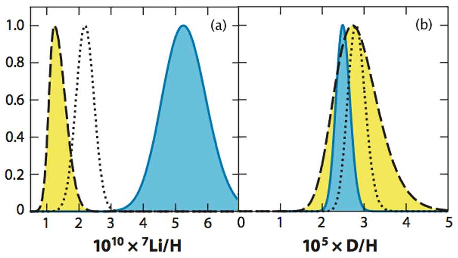
\includegraphics[width=\textwidth]{figures/lithium.pdf}
    \end{columns}
\end{frame}

\begin{frame}
    \frametitle{Cosmology in 2024}
    \begin{columns}
        \column{0.5\textwidth}
        \begin{itemize}
            \item 2024 was a big year for cosmology, with new data releases from multiple surveys:
                \begin{description}
                    \item[Jan] DESY5 SNe:  Improved supernova measurements from the Dark Energy Survey. \hfill \arxiv{2401.02929}
                    \item[Feb] eROSITA: First all-sky survey results from the extended ROentgen Survey with an Imaging Telescope Array. \hfill \arxiv{2402.08458}
                    \item[Mar] DESI:  First year cosmology results from the Dark Energy Spectroscopic Instrument. \hfill \arxiv{2404.03002}
                \end{description}
        \end{itemize}
        \column{0.5\textwidth}
        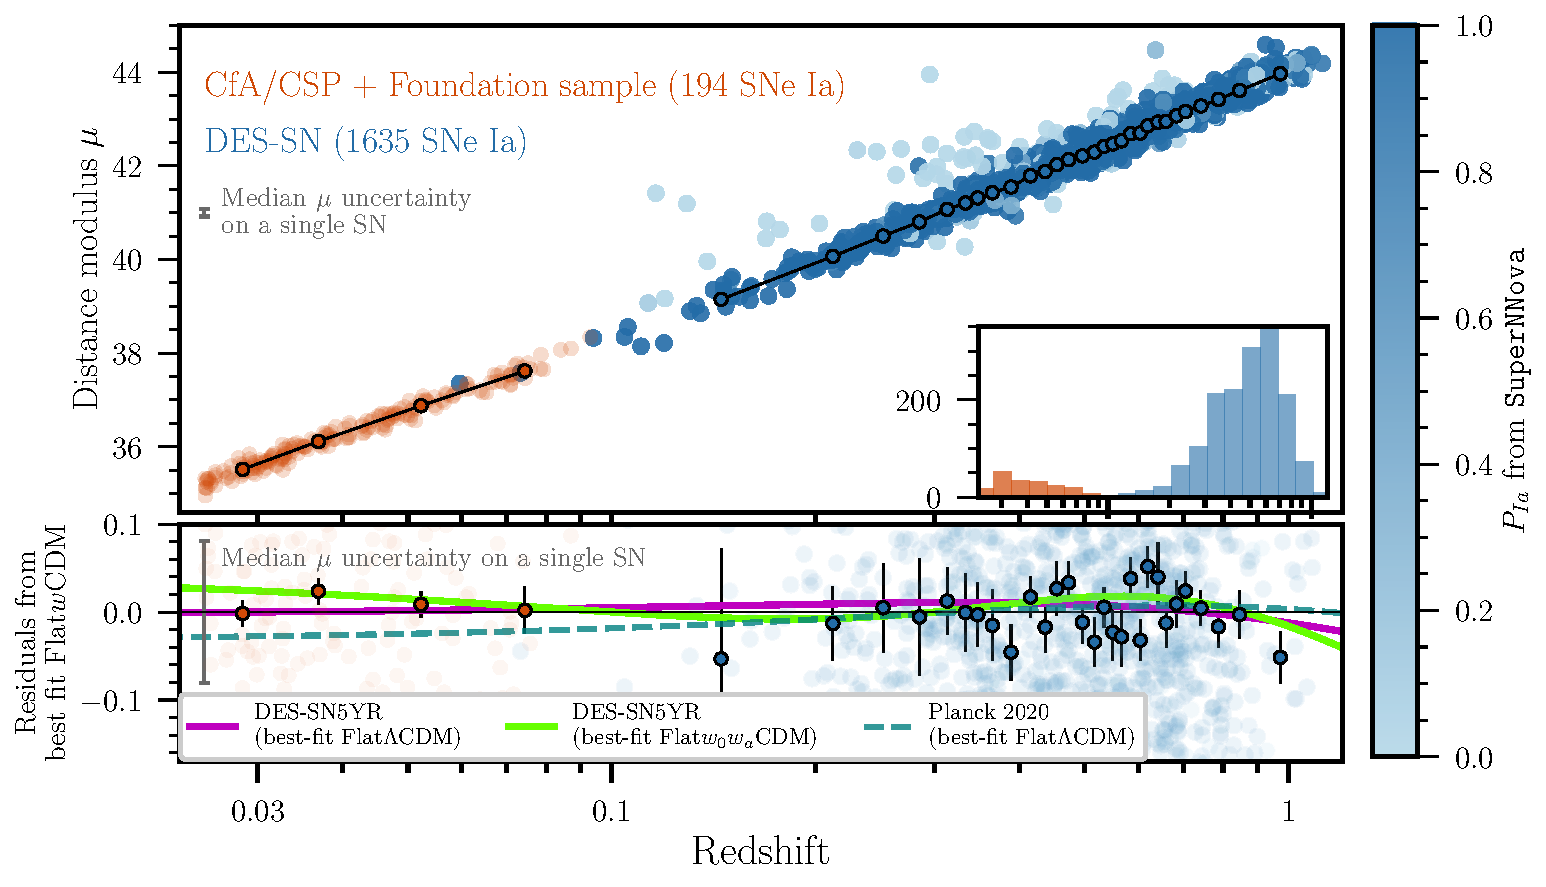
\includegraphics[width=\textwidth]{figures/HD_5yr_KeyPaper.pdf}
        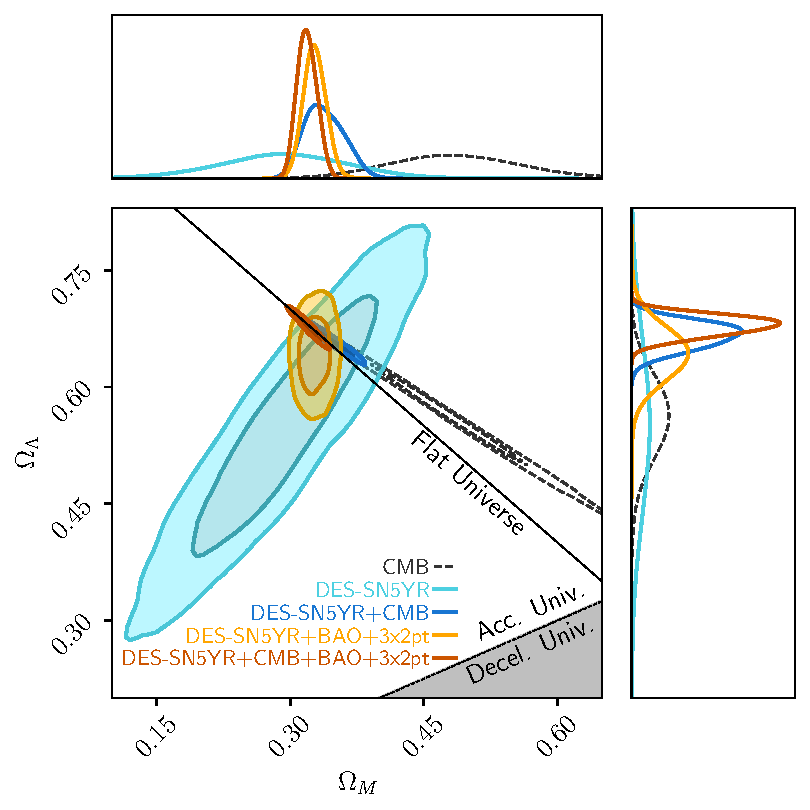
\includegraphics[height=0.42\textwidth]{figures/LCDM_paper.pdf}%
        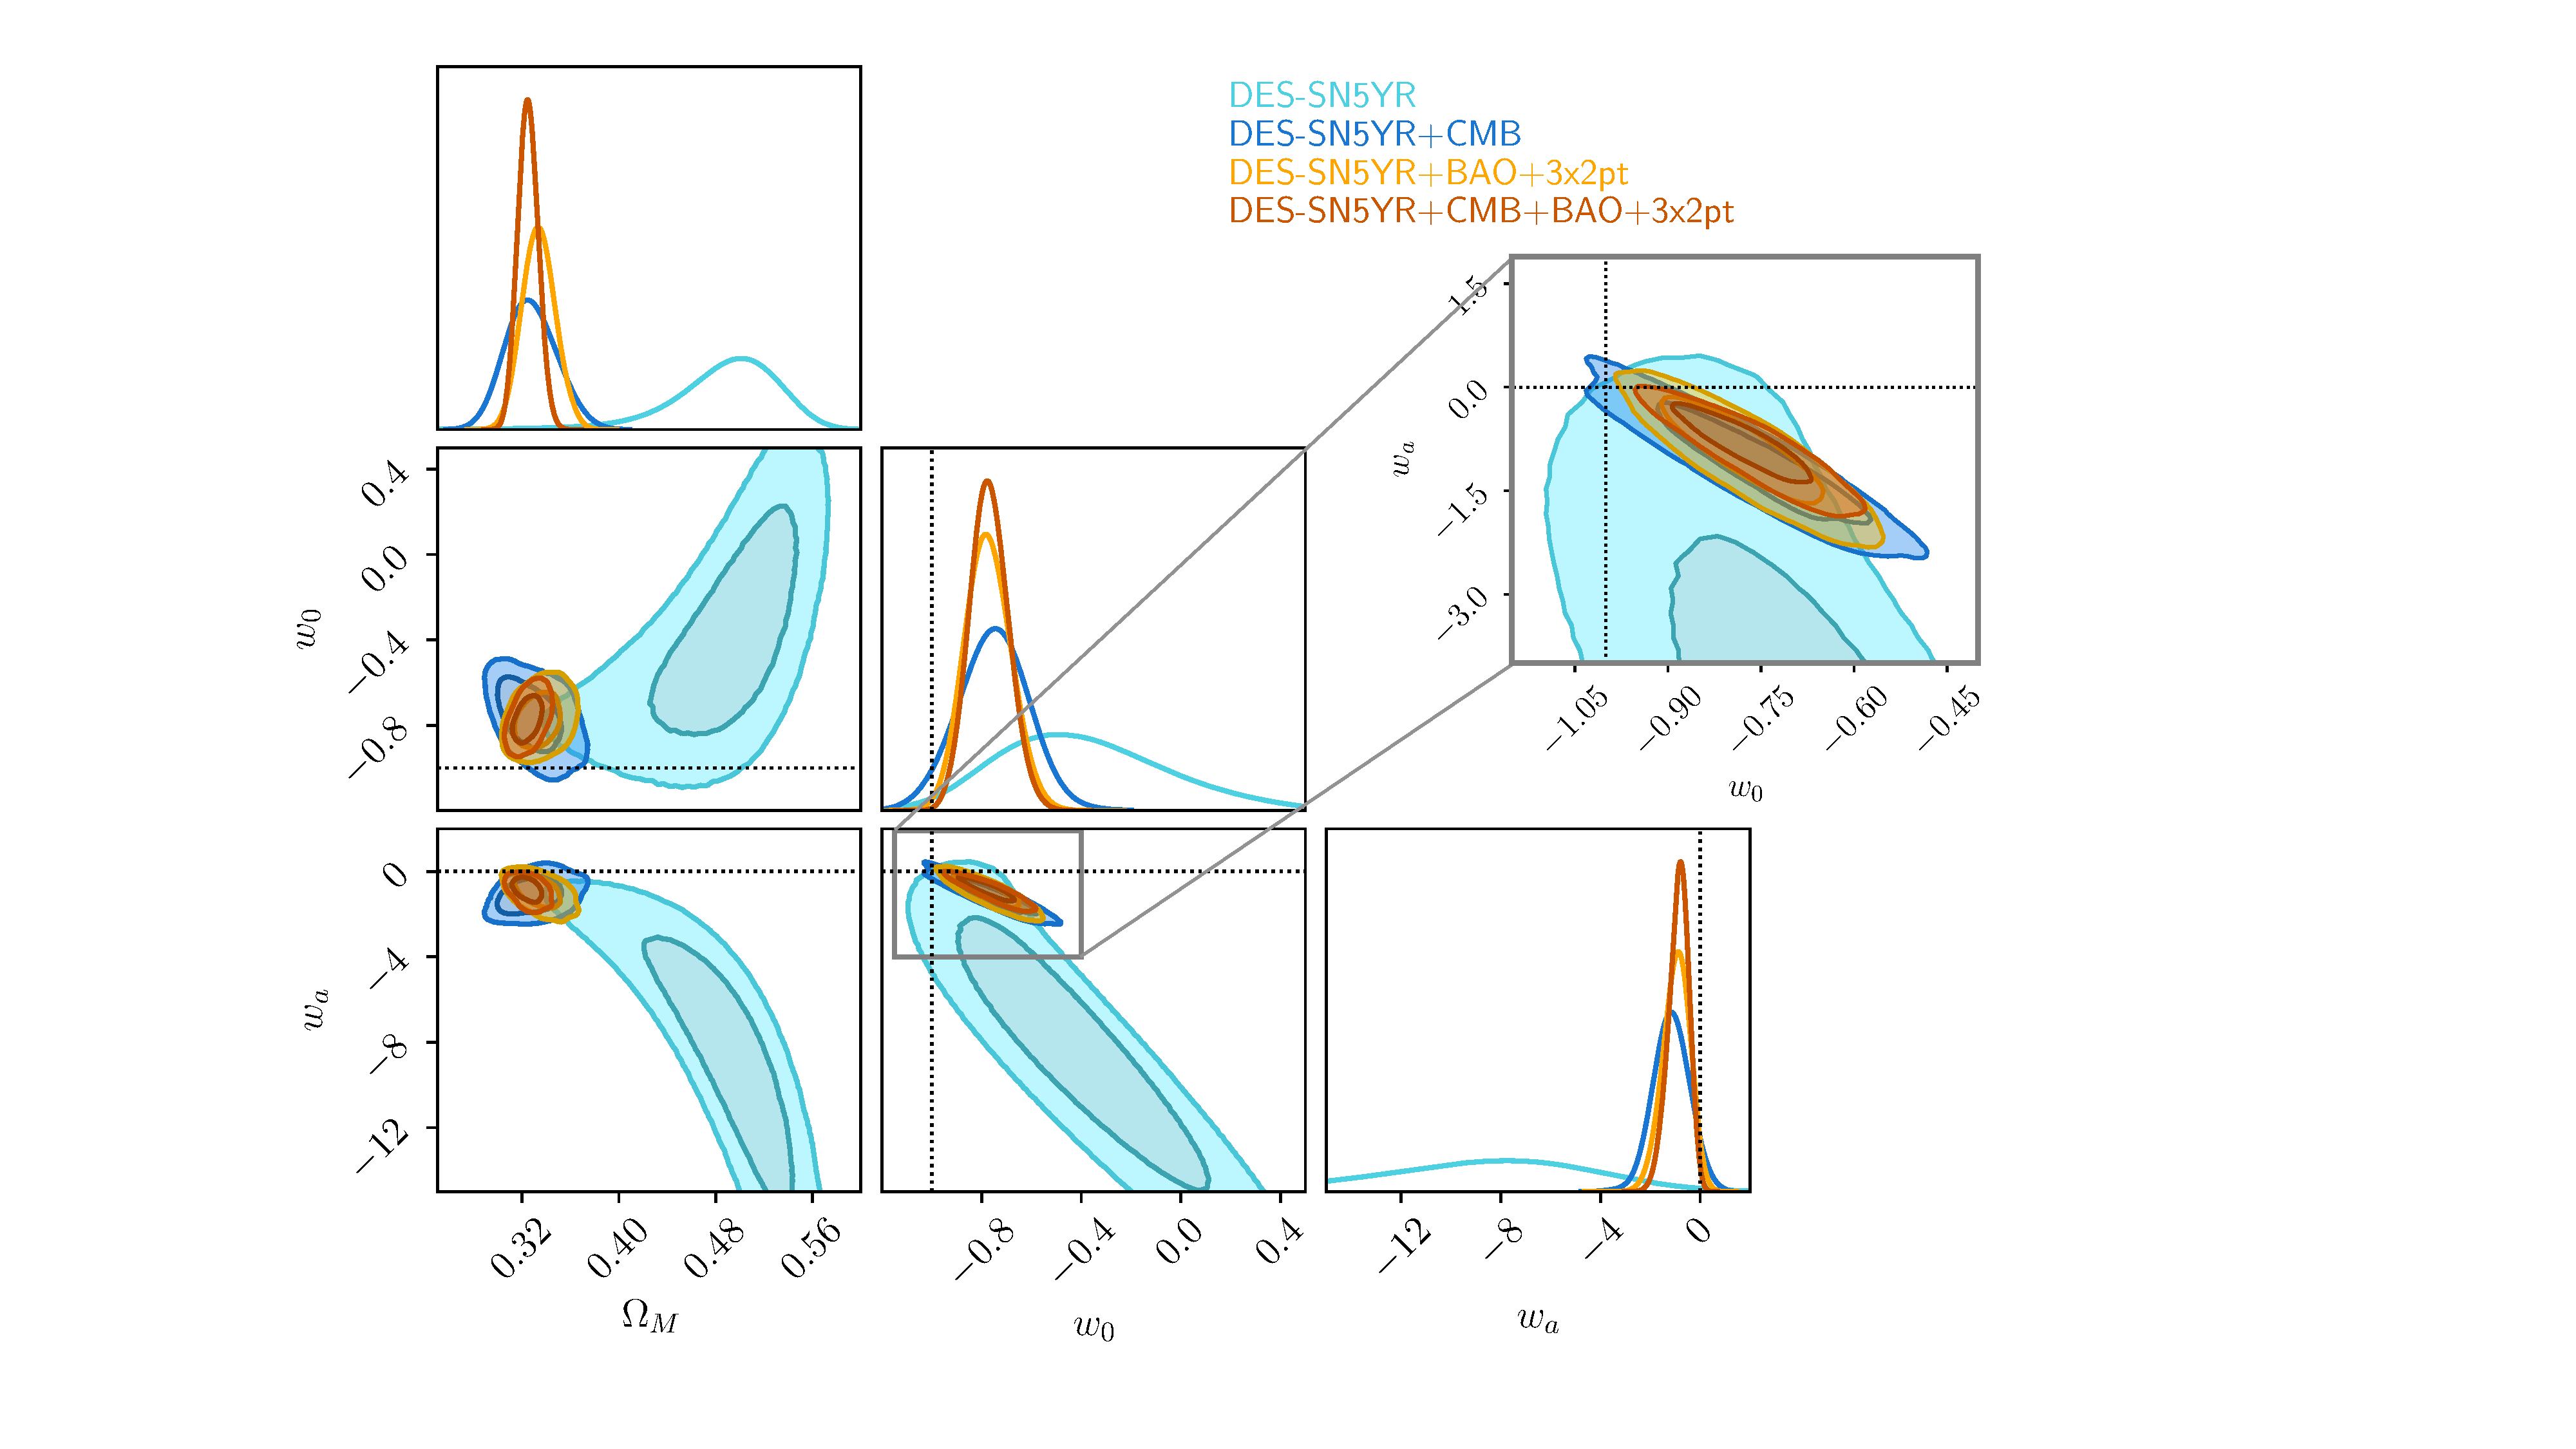
\includegraphics[height=0.42\textwidth]{figures/w0wa_paper_wZoom.pdf}
    \end{columns}
\end{frame}

\begin{frame}
    \frametitle{eROSITA}
    \begin{columns}
        \column{0.5\textwidth}
        \begin{itemize}
            \item eROSITA performed the first all-sky survey in X-rays since ROSAT.
            \item Detected $\sim$12,000 galaxy clusters, providing a powerful new dataset for cosmology.
            \item Results broadly consistent with $\Lambda$CDM, but with some hints of tension in $\sigma_8$. \hfill \arxiv{2402.08458}
        \end{itemize}
        \column{0.5\textwidth}
        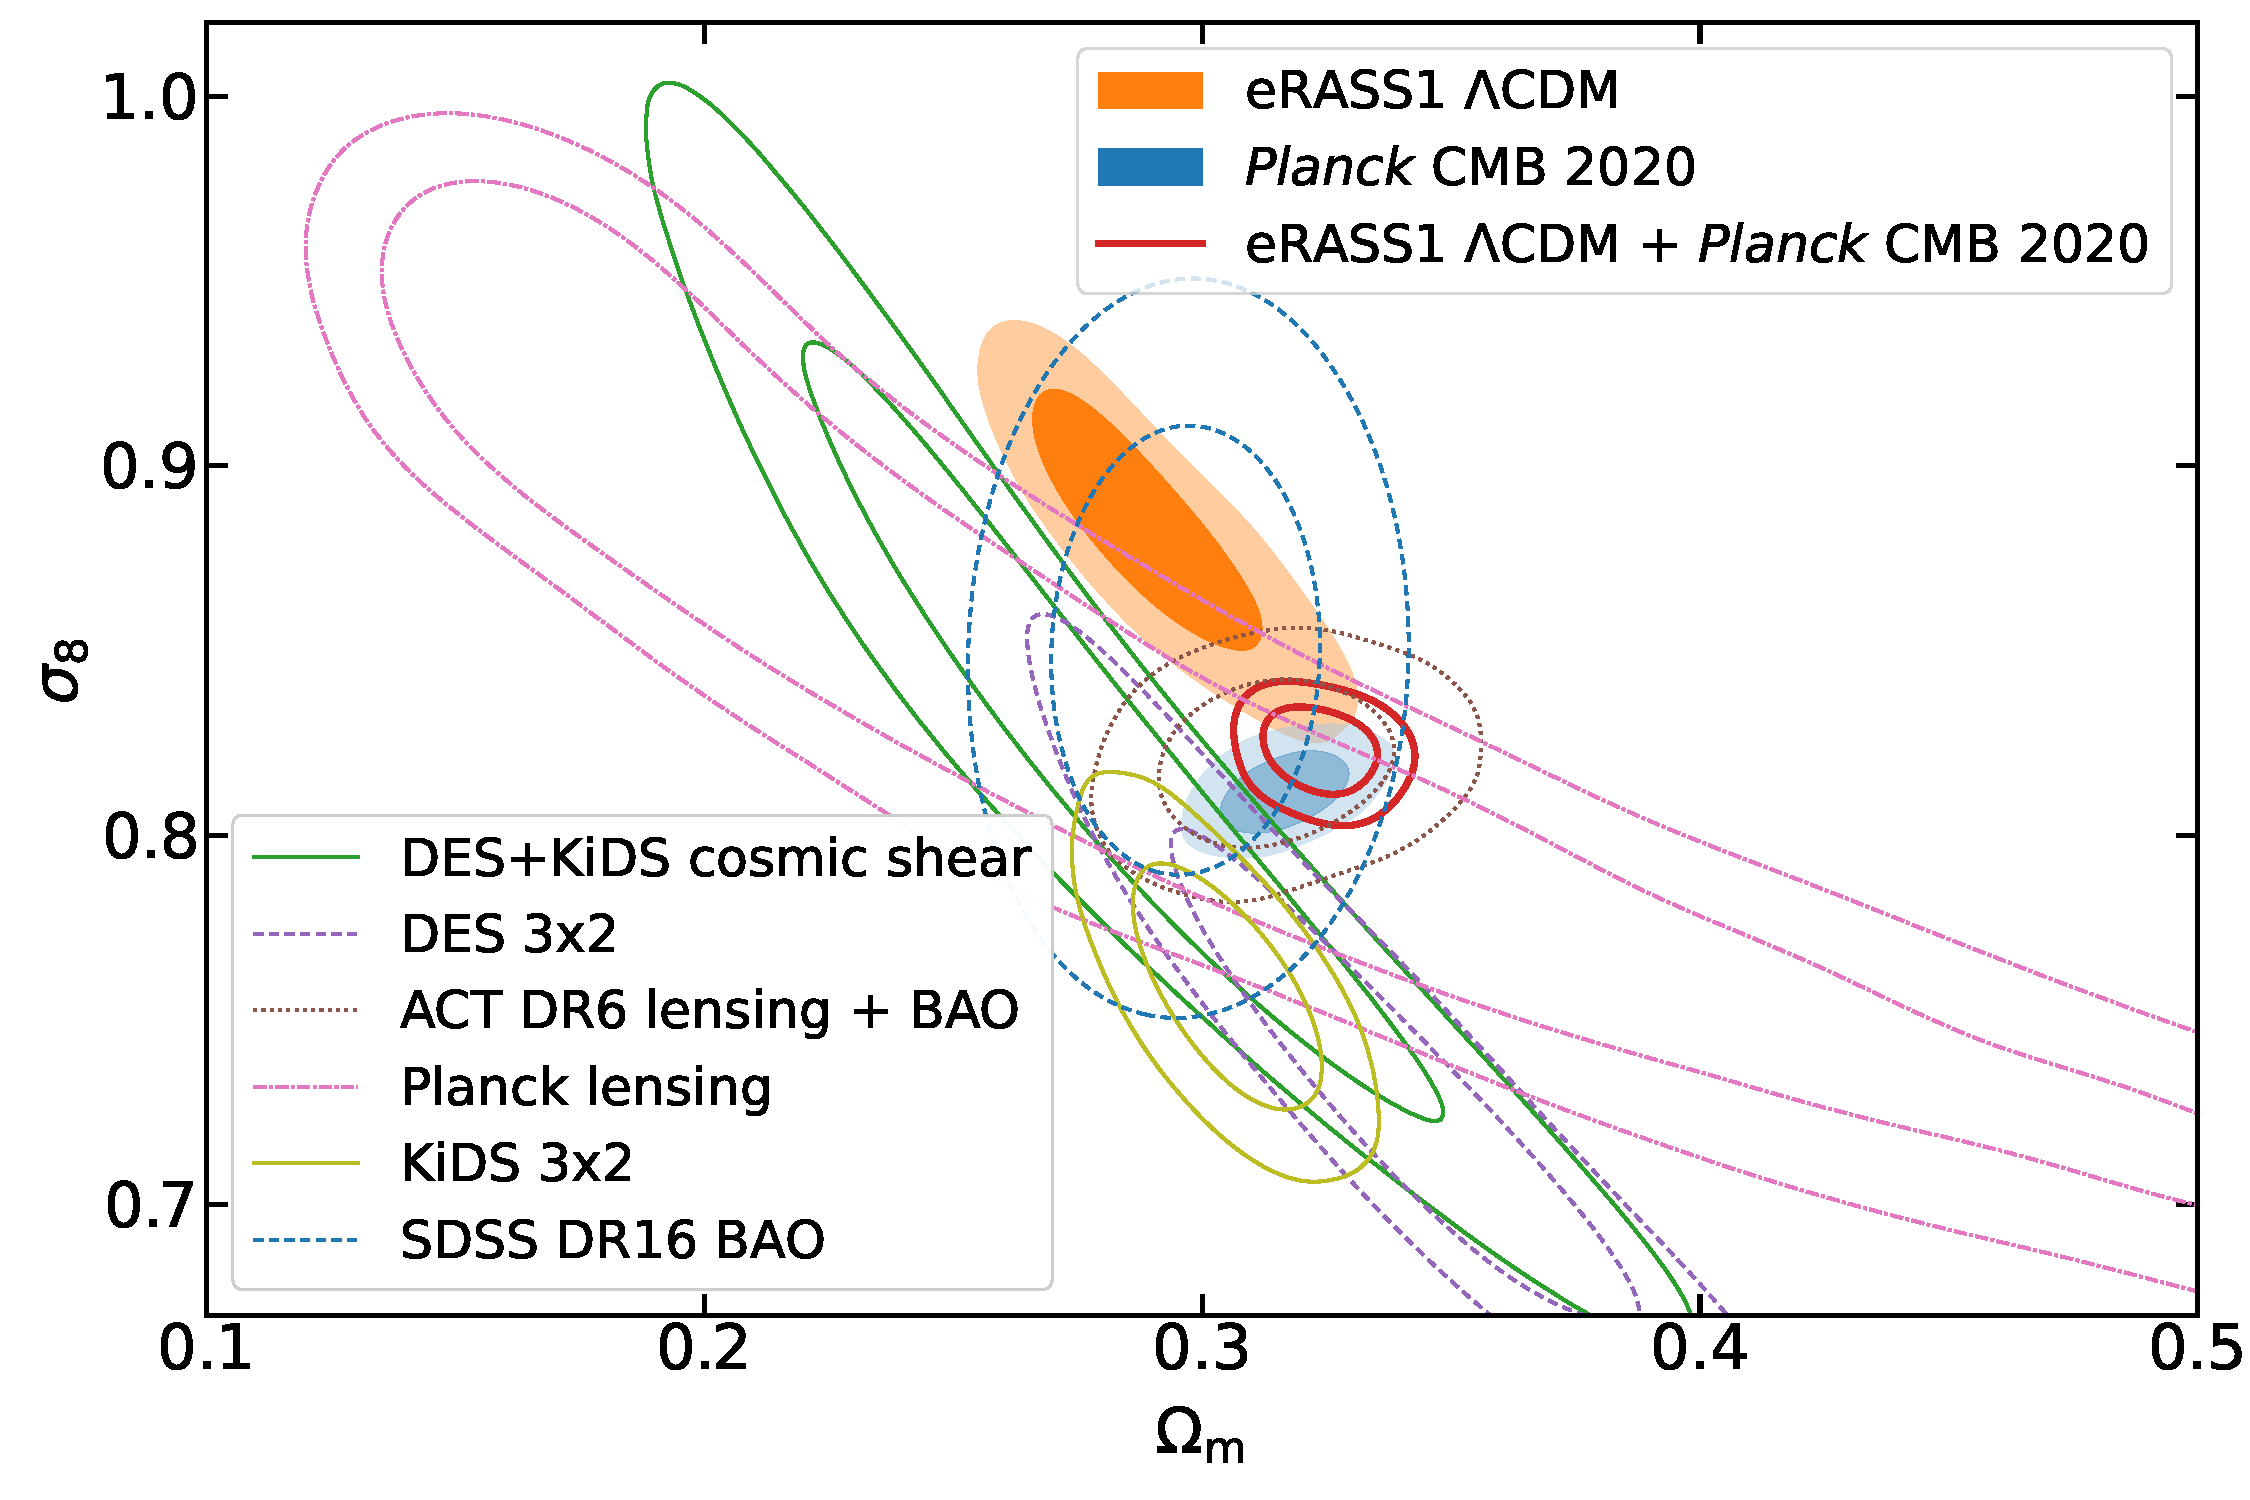
\includegraphics[width=\textwidth]{figures/eROSITA.pdf}
    \end{columns}
\end{frame}

\begin{frame}
    \frametitle{DESI}
    \begin{columns}
        \column{0.5\textwidth}
        \begin{itemize}
            \item DESI is mapping millions of galaxies and quasars to measure BAO and redshift-space distortions.
            \item First year cosmology results strengthen evidence for dark energy, but do not resolve the $H_0$ tension. \hfill \arxiv{2404.03002}
            \item Full BAO and BBN analysis yields $H_0 = 68.53 \pm 0.80$ km/s/Mpc (independent of CMB). \hfill \arxiv{2404.03000}
        \end{itemize}
        \column{0.5\textwidth}
        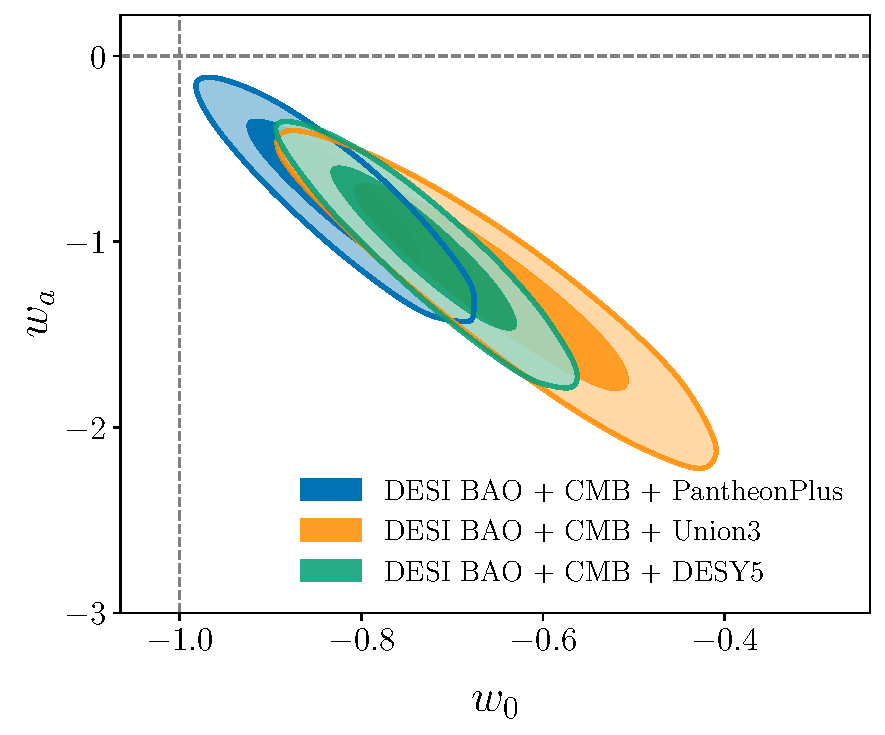
\includegraphics[width=\textwidth]{figures/w0wa_DESI-Planck-SN-95lim.pdf}
    \end{columns}
\end{frame}

\begin{frame}
    \frametitle{What to watch out for}
    \begin{columns}
        \column{0.33\textwidth}
        \begin{itemize}
            \only<1>{
            \item In 2025:
                \begin{itemize}
                    \item DESI: Year 3 BAO results with increased precision.
                    \item DES/Euclid: Improved weak lensing measurements with larger sky coverage.
                    \item eROSITA: Further analysis of X-ray cluster data, including mass calibration.
                    \item ACT: Final data release with improved CMB polarization measurements.
                    \item LVK: Continued gravitational wave observations, potentially increasing the number of standard sirens.
                \end{itemize}
            }
            \only<2>{
            \item Next 5 years:
                \begin{itemize}
                    \item Simons Observatory: High-precision CMB observations, targeting primordial B-modes.
                    \item Rubin: First light and early strong lensing discoveries.
                    \item Roman: Hubble 3.0 with improved Cepheid measurements.
                    \item IPTA: Improved pulsar timing array data, constraining the stochastic gravitational wave background.
                \end{itemize}
            }
            \only<3>{
            \item Next 10-20 years:
                \begin{itemize}
                    \item LISA/Einstein Telescope: Next-generation gravitational wave observatories, probing the early Universe.
                    \item SKA: Large FRB surveys, constraining cosmological parameters and the intergalactic medium.
                    \item LiteBird: Space-based CMB polarization measurements, targeting primordial B-modes.
                    \item ATHENA: High-resolution X-ray observations of galaxy clusters, mass calibration.
                \end{itemize}
            }
        \end{itemize}
        \column{0.67\textwidth}
       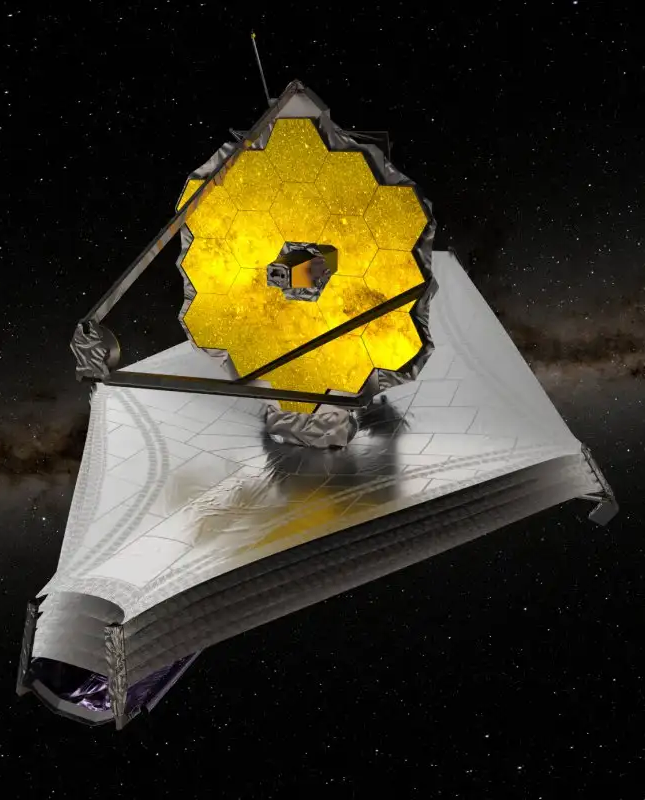
\includegraphics[height=0.145\textwidth]{figures/telescopes/jwst.png}%
        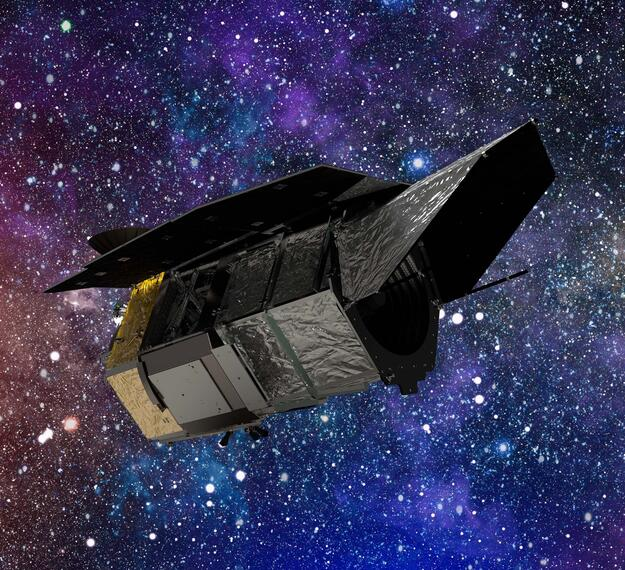
\includegraphics[height=0.145\textwidth]{figures/telescopes/roman.jpg}%
        \includegraphics[height=0.145\textwidth]{figures/telescopes/euclid.jpeg}%
        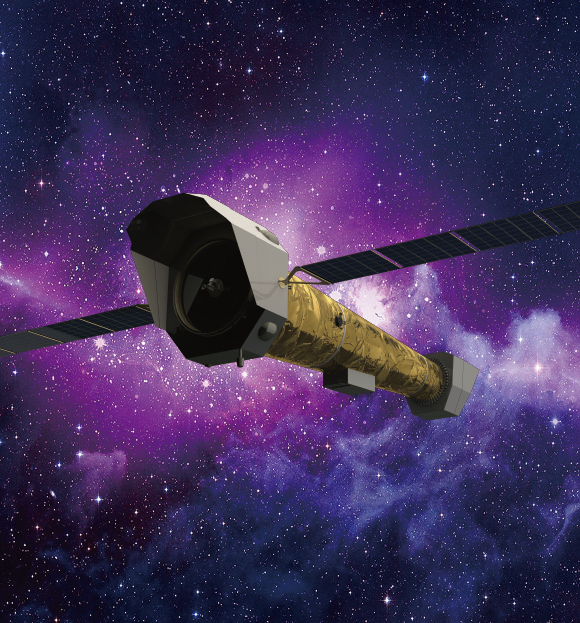
\includegraphics[height=0.145\textwidth]{figures/telescopes/athena.jpg}%
        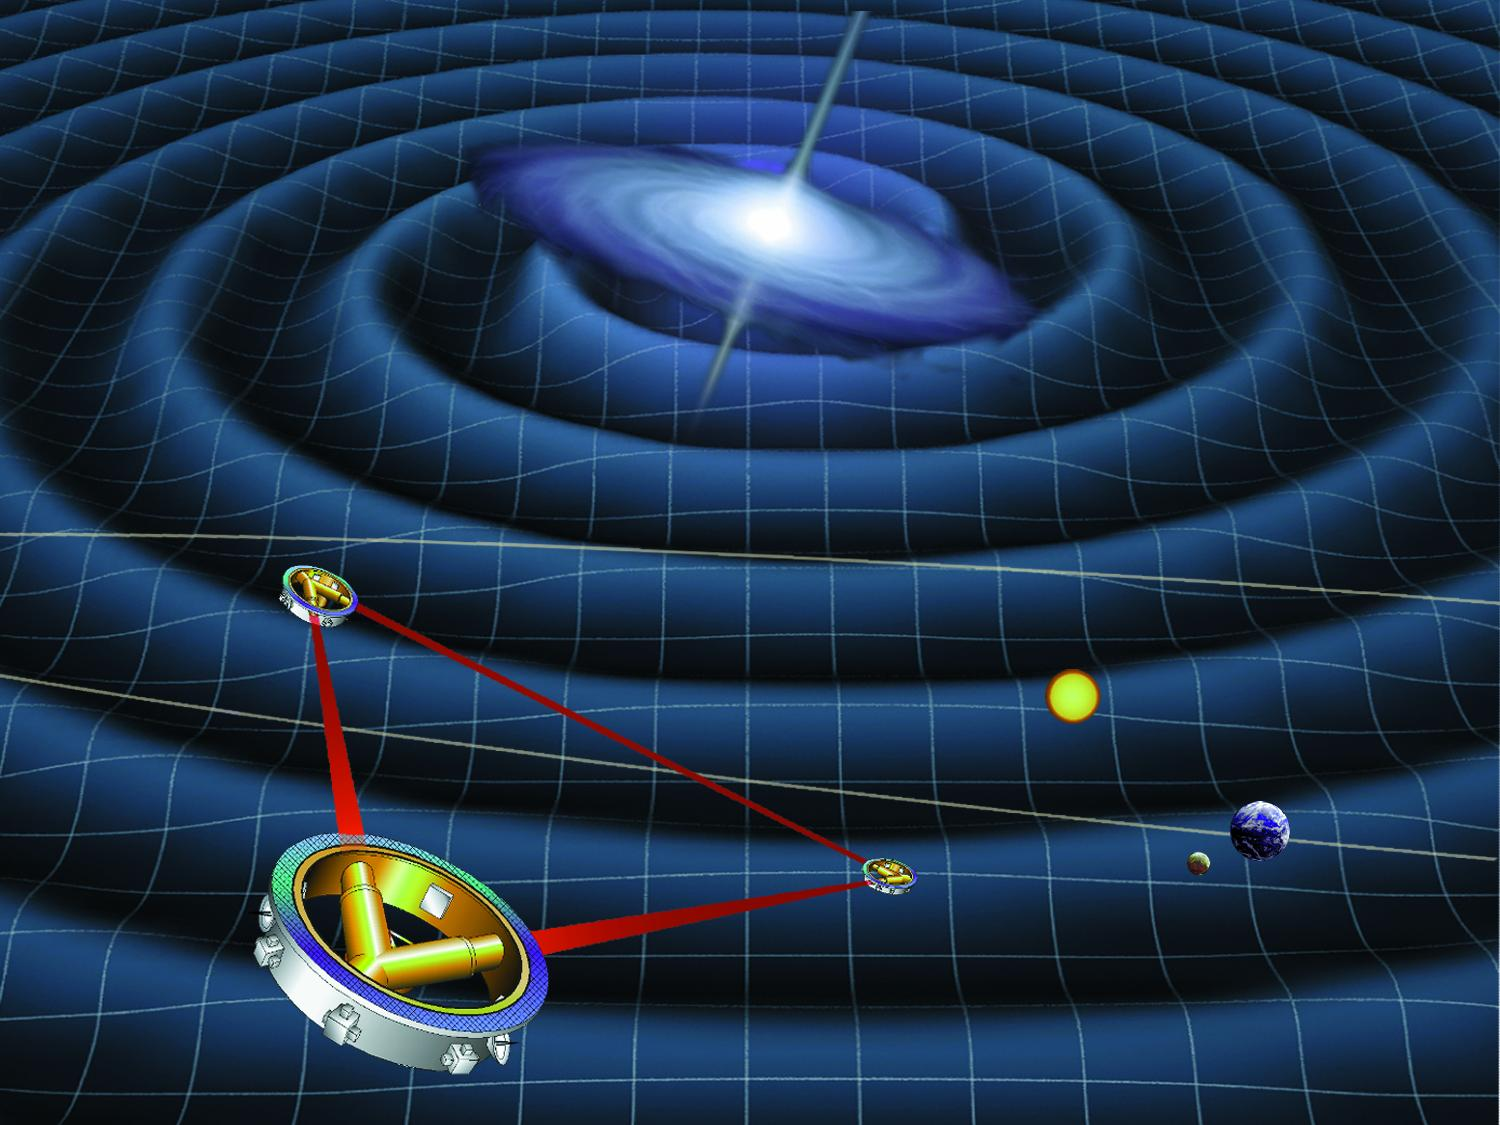
\includegraphics[height=0.145\textwidth]{figures/telescopes/lisa.jpg}%
        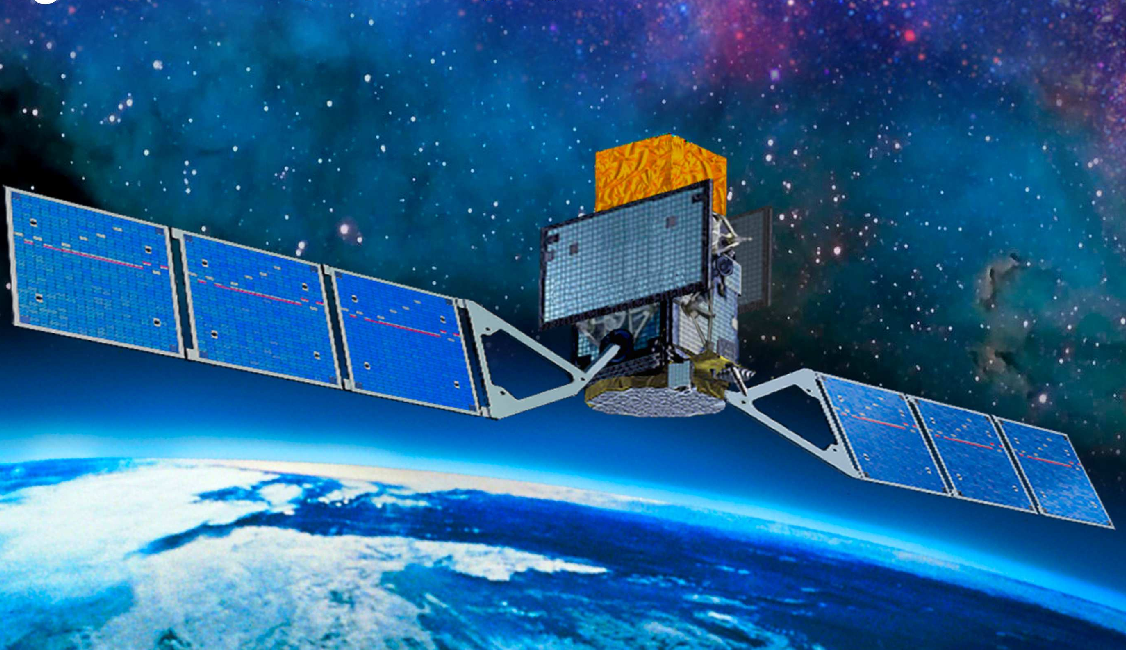
\includegraphics[height=0.145\textwidth]{figures/telescopes/e-ASTROGAM.pdf}%
        \vspace{-1pt}
        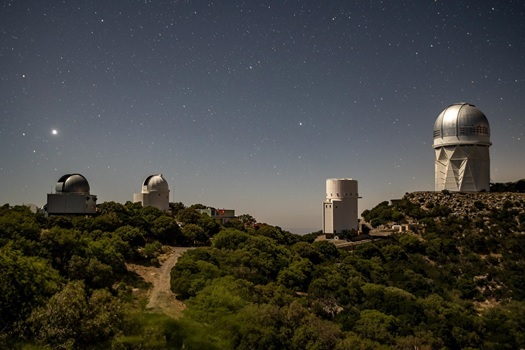
\includegraphics[height=0.15183\textwidth]{figures/telescopes/desi.jpg}%
        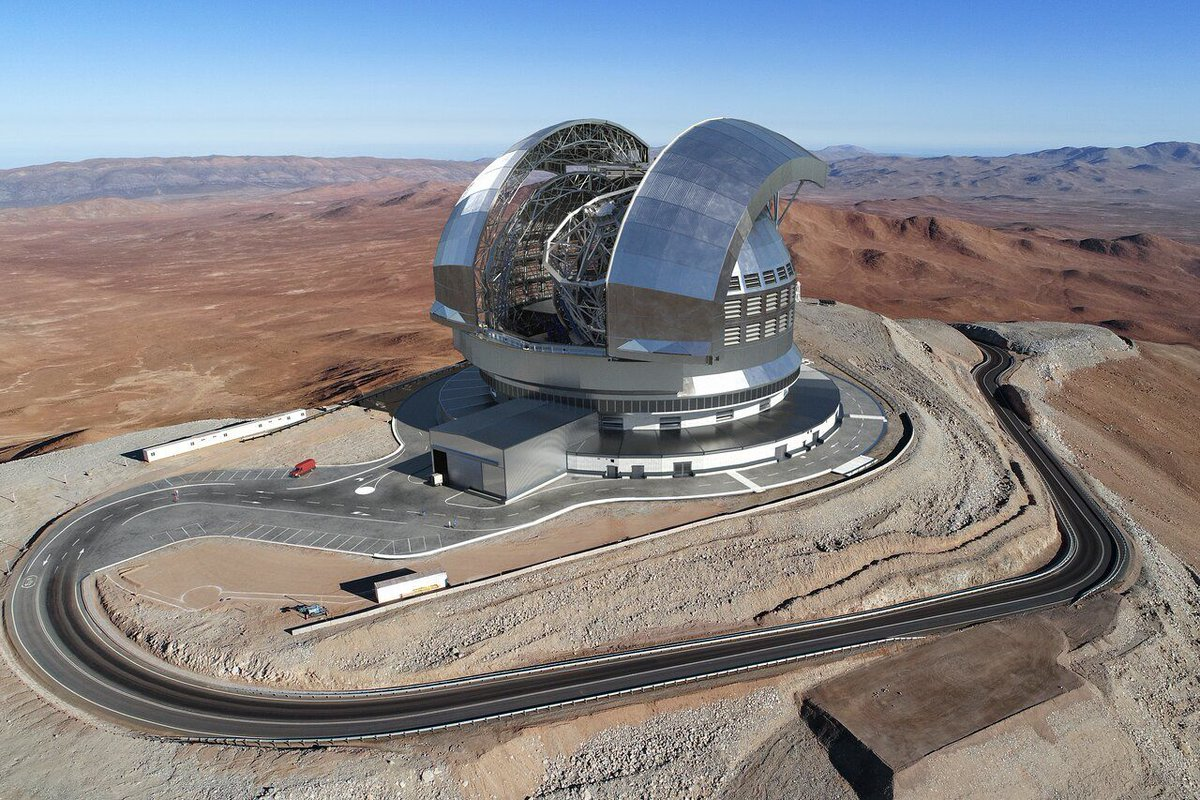
\includegraphics[height=0.15183\textwidth]{figures/telescopes/eelt.jpg}%
        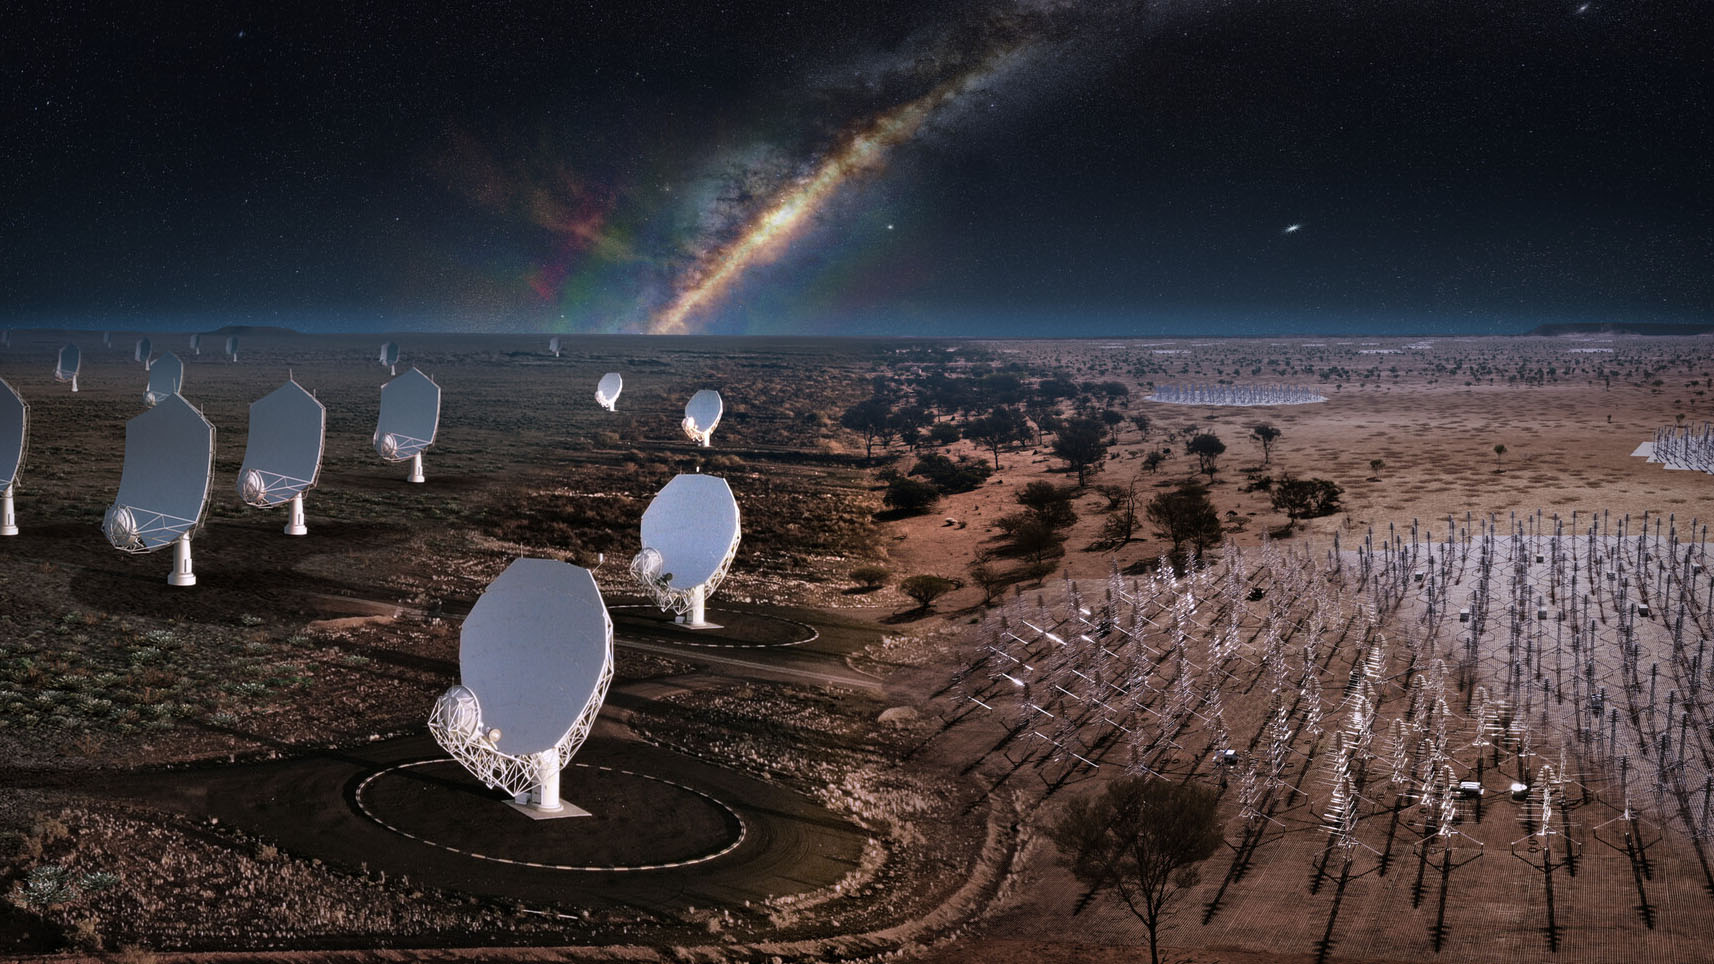
\includegraphics[height=0.15183\textwidth]{figures/telescopes/ska.jpg}%
        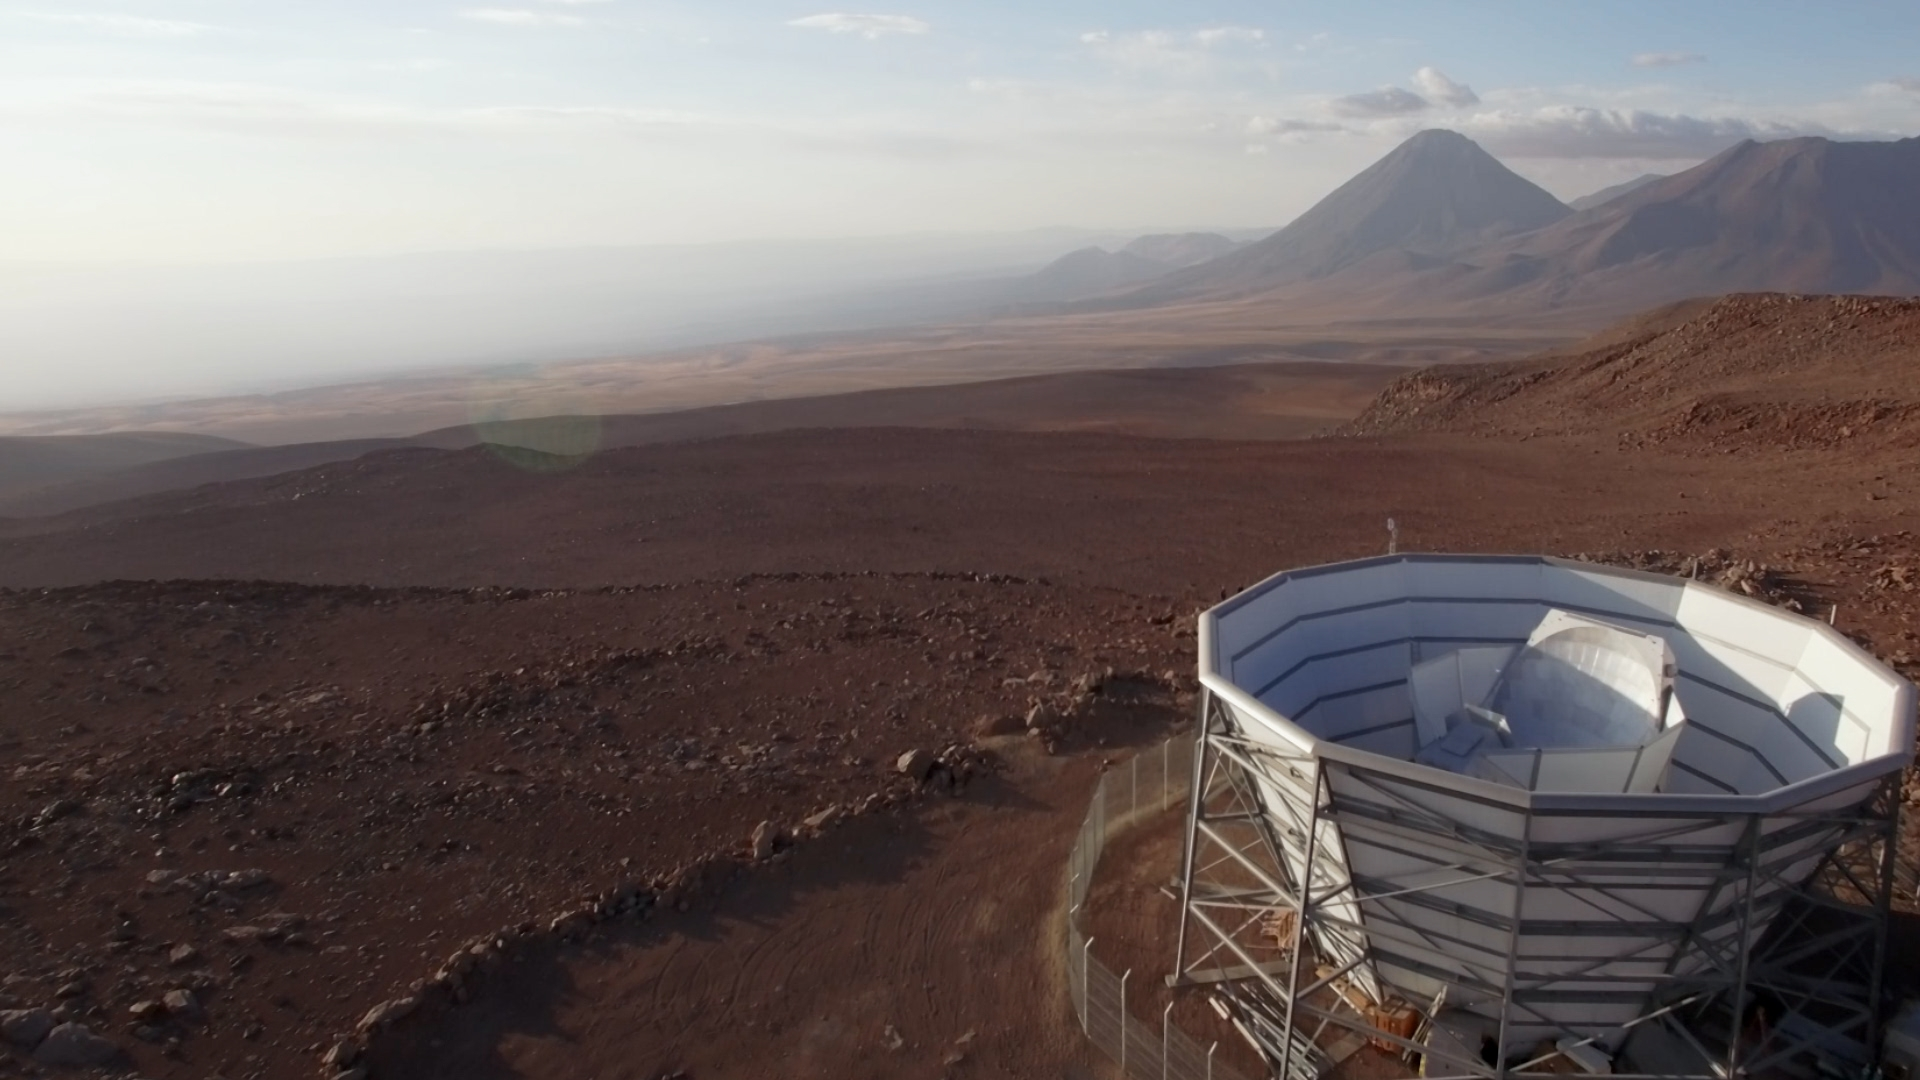
\includegraphics[height=0.15183\textwidth]{figures/telescopes/SO.jpg}%
        \vspace{-1pt}
        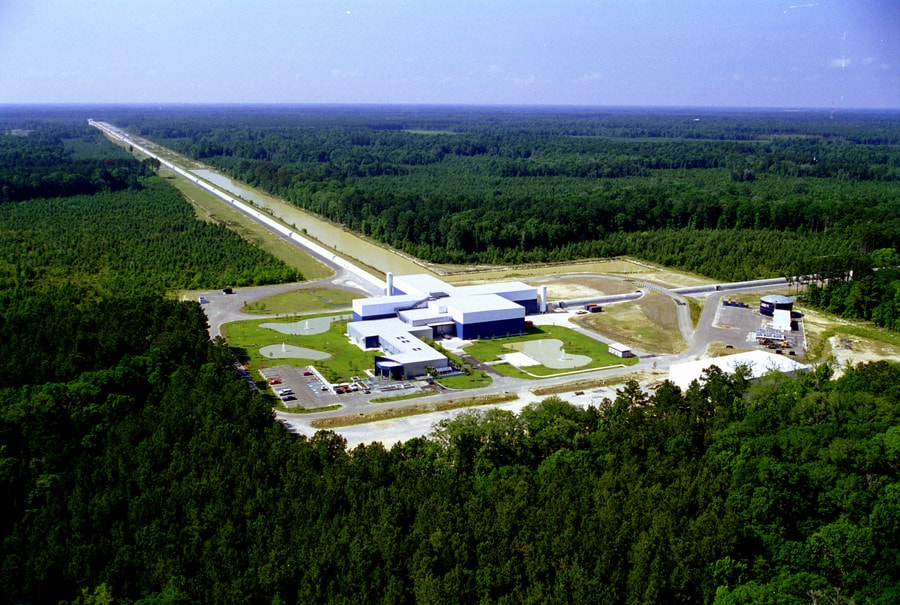
\includegraphics[height=0.18428\textwidth]{figures/telescopes/ligo.jpg}%
        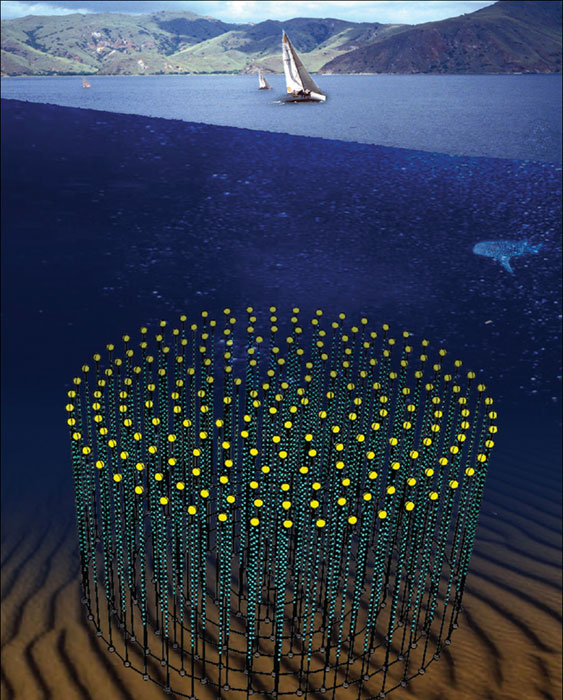
\includegraphics[height=0.18428\textwidth]{figures/telescopes/km3n.jpg}%
        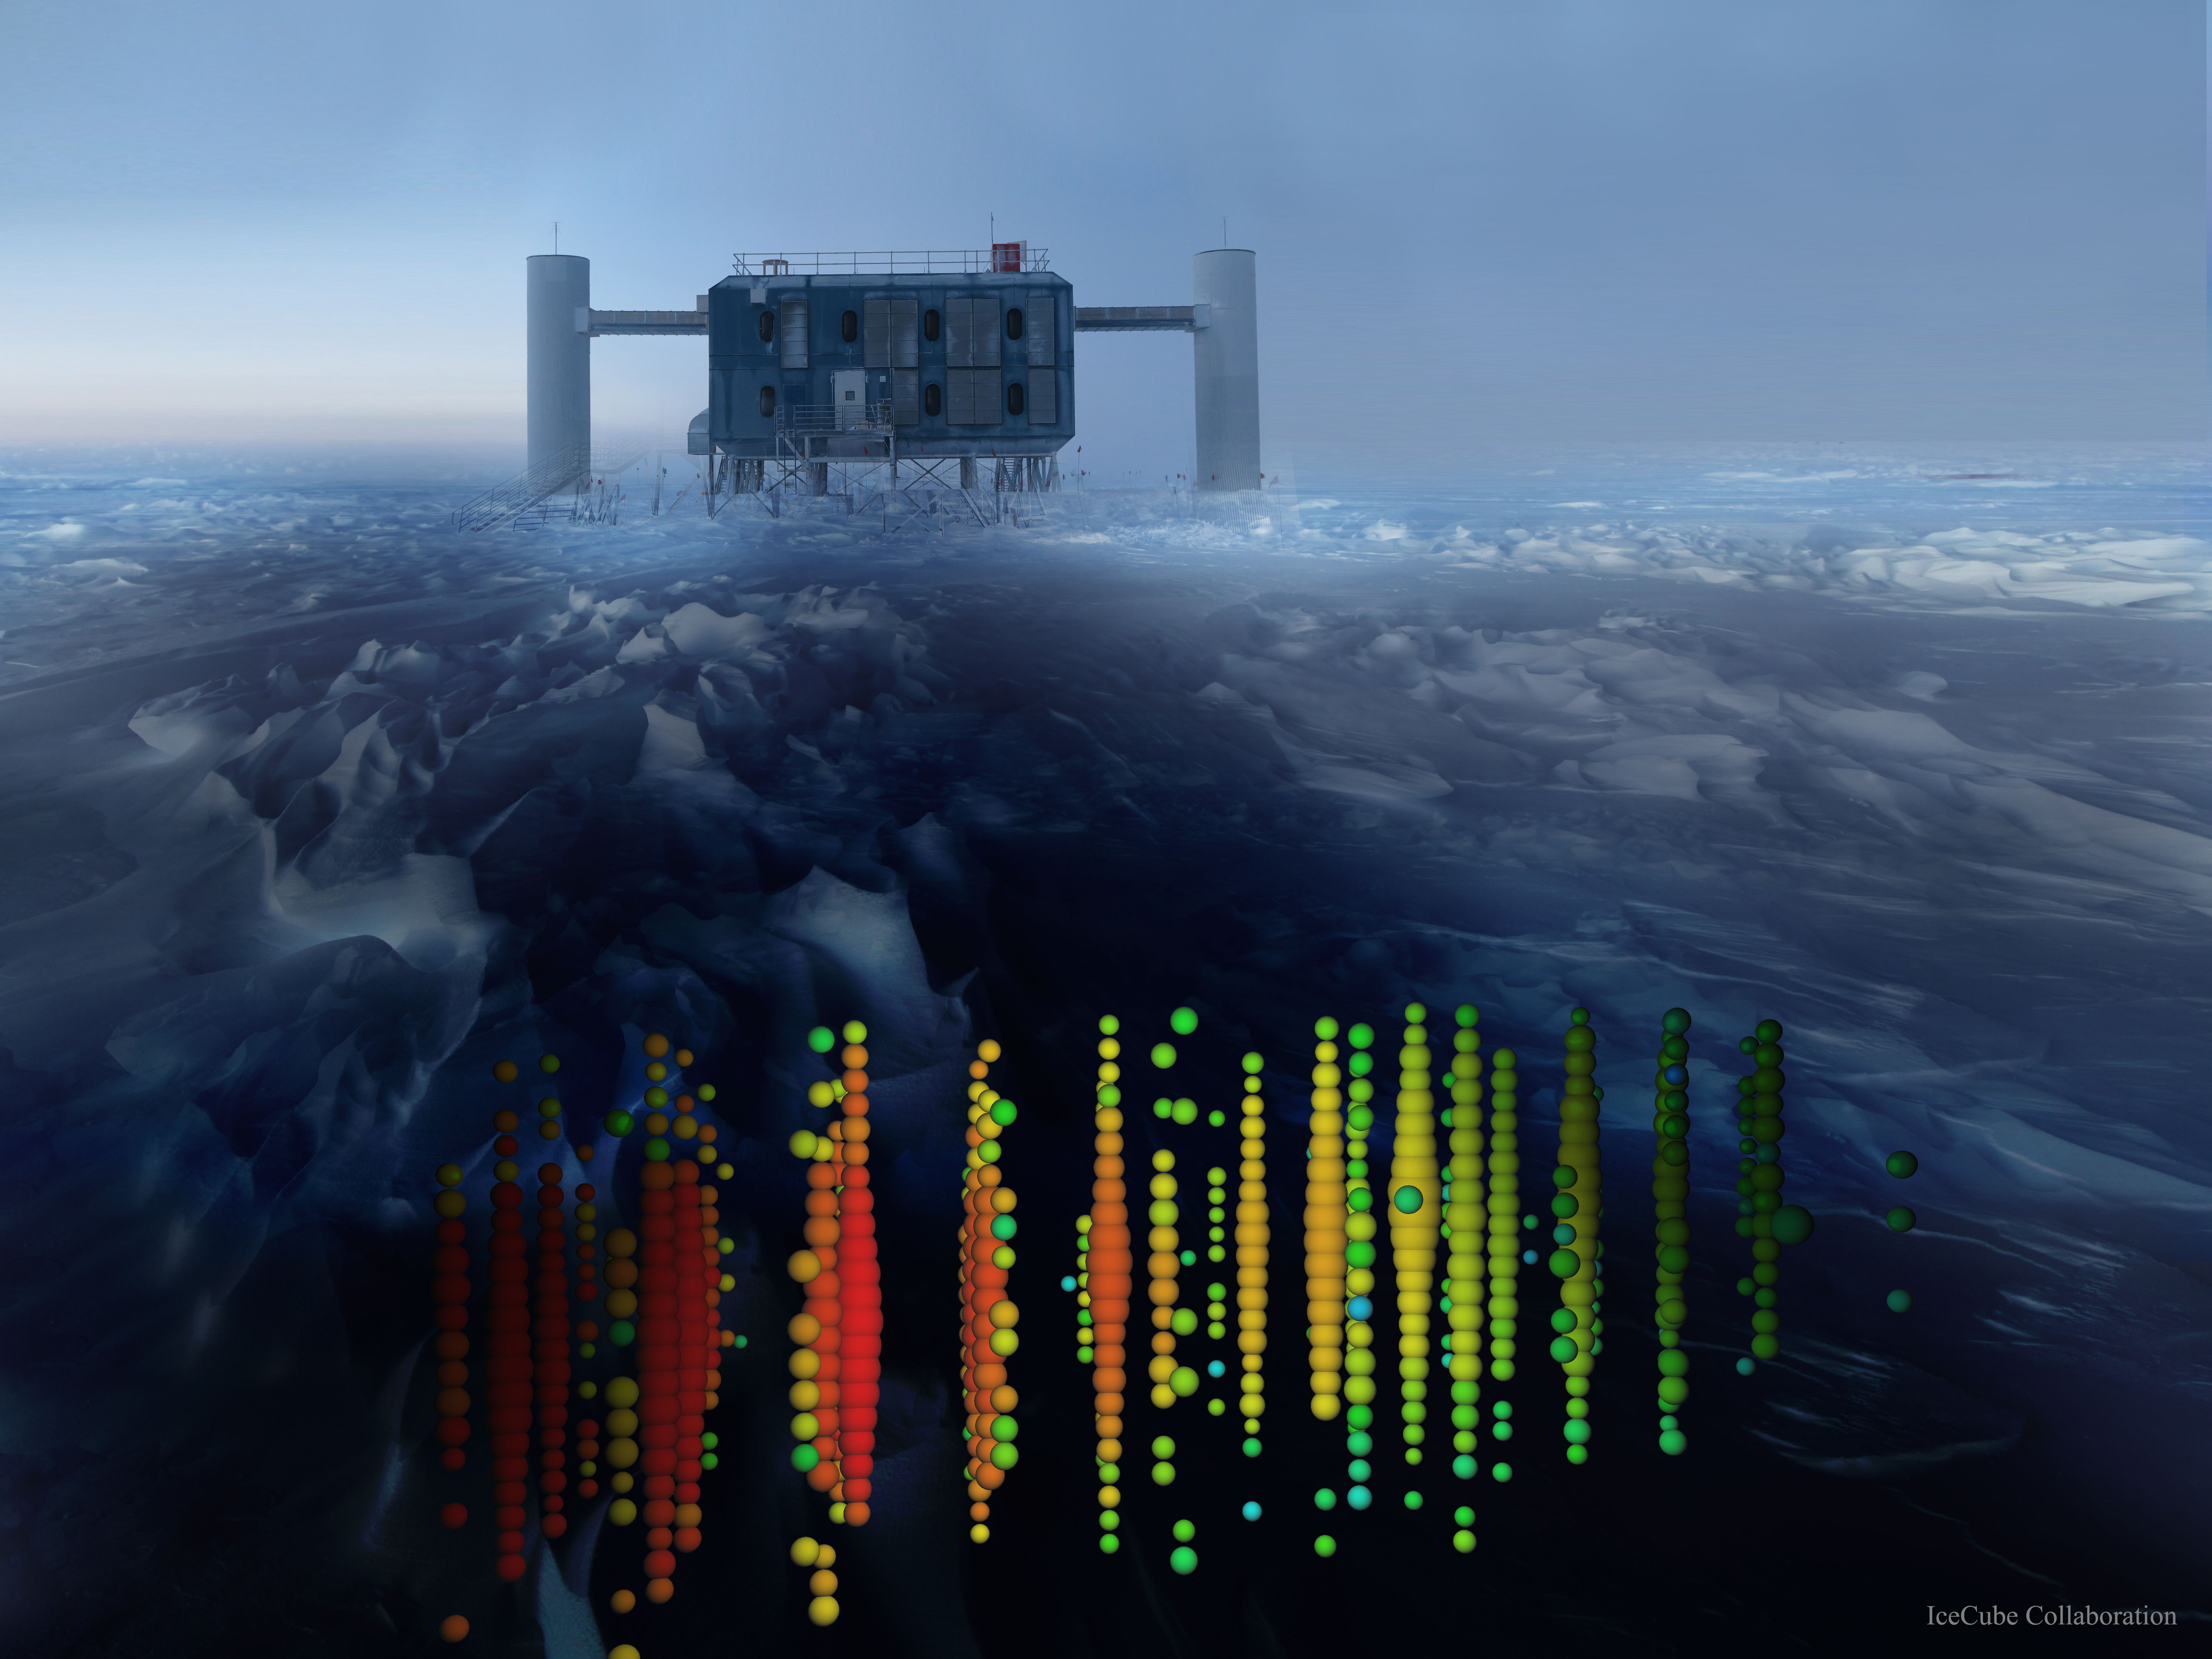
\includegraphics[height=0.18428\textwidth]{figures/telescopes/icecube.jpg}%
        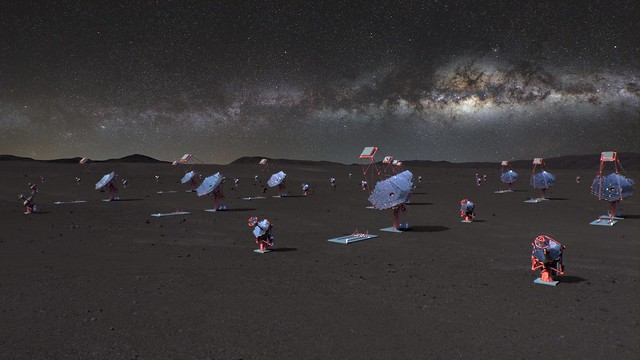
\includegraphics[height=0.18428\textwidth]{figures/telescopes/CTA.jpg}%
    \end{columns}
\end{frame}

\end{document}
